%!TEX root = ../main.tex

\section{Modeling of factor returns} % (fold)
\label{sec:modeling_of_factor_returns}

% Why a model?
This section presents our model for the joint behavior of returns. A multivariate model of returns allows us to make conditional forecasts of the distribution of returns one week ahead, which take into account the dependence between factors. The model is used in the mean-variance analysis, to provide dynamic inputs that can give us optimal weights over time. The model is also used in the analysis of diversification benefits, when we shift the focus to the tail risk of factor portfolios. First, we describe why we choose the copula model among different multivariate models. Second, we define the model and interpret the parameterization. Third, we select and estimate univariate models that are building blocks of the copula. Fourth, we analyze residuals from univariate models, to determine what type of multivariate dependence the copula should capture. Fifth, we estimate the copula and choose the best specification. Last, we conduct a robustness check of whether the copula captures the dependence structure.

%!TEX root = ../main.tex

\subsection{Choosing a multivariate model}
\label{sub:05_01_choosing}
% Why copula?
The ARMA-GARCH family of models has become the norm of modeling univariate financial return series, beginning with \textcite{Bollerslev1986}. The straightforward extension of univariate GARCH models to multiple return series has, however, proven difficult. Unrestricted multivariate GARCH (MGARCH) models that model the conditional covariance matrix directly become impossible to estimate as the number of covariances grows exponentially with the number of series. It thus becomes necessary to restrict the parameter space, where the BEKK model is a common example~\autocite{BEKKModel}.

% Separate modeling of variance and correlation
A parsimonious solution to the dimensionality problem is to separate the modeling of return and volatility dynamics from the modeling of conditional correlations. The separation allows for consistent (albeit inefficient) two-step estimation, and makes large-scale estimation feasible. One such approach is the \emph{dynamic conditional correlation} (DCC) model originally proposed by~\autocite{Engle2002}. In the DCC model, univariate GARCH models are first estimated on each series. Then, an autoregressive process for the correlation matrix is fitted to the standardized residuals ${z_t}$ of those models. 

% Asymmetric cDCC and copula cDCC
DCC is a useful and tractable model for estimating time-varying correlations between return series. However, it is a model of correlations only; it is not flexible enough to model the univariate components differently. More specifically, it is not constructed to generate tail dependence, which is the notion that correlation dynamics can be very different in extreme realizations. 

% Enter the copula
Copula models have recently attracted much attention in the field of risk management, as they provide a flexible way to infer a multivariate probability distribution. Copula models are, just like DCC models, based on two-step estimation and work well in large scale applications. Furthermore, copulas are flexible enough to generate tail dependence, which is shown to be an important feature of factor return data~\autocite{ChristoffersenLanglois2013}. 

Copula models are most often constructed by estimating univariate models from the ARMA-GARCH family in the first step. The residuals from the ARMA-GARCH models are then used in the copula function that explains the multivariate dependence, including dynamic correlations and tail dependence.

Among copula models, there are three main routes of interest: (1) Archimedean copulas, (2) multivariate normal and Student's \textit{t} copulas, and (3) vine copulas. While Archimedean copulas, such as the Gumbel and Clayton specifications, are attractive in many settings, they fail to generate both threshold correlations and simultaneously high unconditional correlations, and are hard to generalize beyond the bivariate case -- making them less attractive for factor return series \textcite{ChristoffersenLanglois2013}. Vine copulas, or pairwise copula constructions, are made up of a combination of bivariate copulas in a tree structure (hence the name vine copulas), and pose an interesting alternative to multivariate normal and Student's \textit{t} copulas. However, the vine method is far less parsimonious as both the number of bivariate combinations and the number of different tree structures increase exponentially with the number of assets modeled \autocite{Aas2009}.

We choose to work with multivariate Student's \textit{t} copula models, as they can (1) estimate the joint distribution function in large scale applications, (2) model different univariate models for the different factors, and (3) incorporate both tail dependence and dynamic correlations. Next, we define and describe the copula model. % motivating the choice of copula, and among copulas

%!TEX root = ../../main.tex

\subsection{Definition of copula model} % (fold)
\label{sub:definition_of_copula_model}

Each week $t$, the conditional joint density of returns on $N$ assets $R_{t+1} = \{r_{i,t+1},\ldots,r_{N,t+1}\}$ is described by a joint density function $f_t(R_{t+1})$. Following~\textcite{ChristoffersenErrunzaJacobLanglois2012}, who build on~\textcite{Patton2006} and~\textcite{Sklar1959}, we decompose the joint density function into the product of a joint copula function $c_t(U_{t+1})$ of uniformly distributed variables $U_{t+1} \sim U(0, 1)$ and marginal densities $f_{i,t}(r_{i,t+1})$:
\begin{align}
  f_t(R_{t+1}) =
    c_t(U_{t+1}) \prod^N_{i=1} f_{i,t}(r_{i,t+1})
  \label{eq:copula_sklar}
\end{align}
The elements of $U_{t+1} = \{u_{i,t+1},\ldots,u_{N,t+1}\}$ are related to the original returns by the probability integral transform, i.e the cumulative distribution of $r_{i,t+1}$:
\begin{align}
  u_{i,t+1} = F_{i,t}(r_{i,t+1}) = \int_{-\infty}^{r_{i,t+1}} f_{i,t}(r)dr
\end{align}
The copula function $c_t(U_{t+1})$ is a multivariate skewed \emph{t} distribution. This distribution is parameterized by a single degrees of freedom parameter $\nu_c$, controlling the degree of dependence, a vector of $N$ skewness parameters $\gamma_c$, controlling the asymmetry in dependence, and a potentially time-varying correlation matrix $\Psi_{t}$.\footnote{We describe the details of the skewed \emph{t} distribution, including the expanded form of $c_t$, in~\autoref{app:ghstmv}.} The skewed \emph{t} distribution nests the standard (hereafter symmetric) \emph{t} distribution when all $\gamma_{i,c} = 0$ and the standard normal distribution when additionally $\nu_c = \infty$.

The log-likelihood of the model is constructed from~\autoref{eq:copula_sklar}:
\begin{align}
  L =
    \underbrace{\sum_{t=1}^T \log(c_t(U_{t+1}))}_\text{Copula} +
    \underbrace{\sum_{t=1}^T \sum_{i=1}^N \log(f_{i,t}(r_{i,t+1}))}_\text{Marginals}
\end{align}
At this point, it is worth noting that the joint density $c_t(U_{t+1})$ need not be of the same family as the marginal densities $f_{i,t}(r_{i,t+1})$ -- nor are we restricted to modeling $f_{i,t}(r_{i,t+1})$ jointly for all factors. In fact, we take advantage of this flexibility and choose to model the marginal densities independently as ARMA-GARCH processes, which allows us to capture a number of predictable features in the univariate series -- serial correlation, volatility clustering and leverage effects. The marginal models are estimated independently by maximizing the likelihood(s) of the second term, and then the copula is estimated by maximizing the first term -- using the residuals of the marginal models as given.

This procedure is called multi-stage maximum log-likelihood or inference functions for margins and greatly simplifies the estimation procedure, while yielding relatively efficient estimates~\autocite{Patton2006,Joe1997}. The modeling and estimation of our ARMA-GARCH models is detailed in the upcoming subsection, whereas the remainder of this subsection describes how we make the correlation matrix $\Psi_t$, and thus the dependence between factors, dynamic.

The copula is made dynamic by fitting a dynamic conditional correlation (DCC) process for $\Psi_t$ to copula residuals $z_{t+1}^*$~\autocite{Engle2002}. Using the notation from~\textcite{ChristoffersenLanglois2013}:
\begin{align}
  Q_t = (1 - \alpha - \beta) Q
    + \beta Q_{t-1}
    + \alpha \bar{z}_{t-1}^* \bar{z}_{t-1}^{*\top}
  \label{eq:copula_cdcc}
\end{align}
where $Q_t$ is normalized to the correlation matrix $\Psi_t$:
\begin{align}
  \Psi_t = Q_t^{-\frac{1}{2}} Q_t Q_t^{-\frac{1}{2}}
  \label{eq:copula_cdcc_psi}
\end{align}
The $Q_t$ process is comprised of three components that are weighted according to $\alpha, \beta$: (1) a time-invariant component: $Q$, (2) an innovation component from copula shocks: $\bar{z}_{t-1}^{*} \bar{z}_{t-1}^{*\top},$\footnote{Where $\bar{z}_{i,t+1}^* = z_{i,t+1}^* \sqrt{q_{ii,t}}$ is due to a correction by~\textcite{Aielli2013}, that improves the reliability of the estimation procedure.} and (3) an autoregressive component of order one: $Q_{t-1}$. In order for the the correlation matrix $\Psi_t$ to be positive definite, $Q_t$ has to be positive definite, which is ascertained by requiring that $\alpha \geq 0$, $\beta \geq 0$ and $(\alpha + \beta) < 1$. The model nests a constant copula when $\alpha = \beta = 0$.

The model for $c_t(U_{t+1})$ is comprised of $1 + N$ distribution parameters $\{\nu_c, \gamma_c\}$ and $2 + \frac{N(N-1)}{2}$ dynamics parameters $\{\alpha, \beta, Q\}$, where the elements of $Q$ are estimated using moment matching, and the remaining parameters $\{\alpha, \beta, \nu_c, \gamma_c\}$ are estimated using maximum likelihood.\footnote{A detailed description of the copula estimation procedure can be found in~\autoref{app:copula_cdcc}.}

ARMA-GARCH modeling allows us to filter time-varying effects, leaving independent \emph{standardized residuals} $z_{i,t}$, which are assumed to follow a constant distribution $f_i(z_{i,t})$. These residuals are first transformed into uniform variables $u_{i,t+1}$ by the probability integral transform of the densities above, and then made to follow the \emph{copula} distribution by the \emph{inverse} probability integral transform of the \emph{copula}:
\begin{align}
  z_{i,t+1}^* = F^{-1}_{\nu_c,\gamma_{i,c}}(F_{i}(z_{i,t+1}))
\end{align}

The interpretation of the copula parameterization is closely associated to the structure of multivariate dependence. By different restrictions on the parameters in the DAC model, we are able to activate or deactivate certain features of the copula: First, the degree of freedom parameter $\nu_c$ is to be interpreted as the measure of tail dependency. When $\nu \neq 0$, the lower and upper tails of the joint distribution are fatter than in the normal case, which is coherent with earlier evidence of threshold correlations~\autocite{ChristoffersenLanglois2013}. Second, the skewness parameters $\gamma_{c,i}$ are to be interpreted as the extent of asymmetry in the correlation structure. When $\gamma \neq 0$, there is asymmetry in correlations. Third, the $\alpha$ and $\beta$ parameters determine whether the copula generates time-varying correlations. If $\alpha \neq 0$ and $\beta \neq 0$, the copula is dynamic. An overview of the six copula models is given in \autoref{tab:conceptual}.

%!TEX root=../../main.tex

\begin{table}
  \centering
  \footnotesize
  \renewcommand{\arraystretch}{1.2}

  \caption{Conceptual matrix of copula parameterizations}

  \begin{tabularx}{0.80\textwidth}{@{} lc c >{\centering}Xc >{\centering}Xc >{\centering\arraybackslash}X}
    \toprule
      & && \textbf{Normal} && \textbf{Symmetric \emph{t}} && \textbf{Skewed \emph{t}} \\
      \cmidrule{4-4}
      \cmidrule{6-6}
      \cmidrule{8-8}
      & && $\nu_c = \infty$   && $\nu_c < \infty$   && $\nu_c < \infty$ \\
      & && $\gamma_{i,c} = 0$ && $\gamma_{i,c} = 0$ && $\gamma_{i,c} \neq 0$ \\
      \cmidrule{4-8}
    \cmidrule{1-2}
    \multirow{2}{*}{\textbf{Constant}} & $\alpha = 0$ && Constant && Constant && Constant \\
                              & $\beta = 0$  && Normal   && Symmetric \emph{t} && Skewed \emph{t}      \\
    \cmidrule{1-2}
    \multirow{2}{*}{\textbf{Dynamic}}  & $\alpha > 0$ && Dynamic  && Dynamic && Dynamic \\
                              & $\beta > 0$  && Normal   && Symmetric \emph{t} && Skewed \emph{t}      \\
    \bottomrule
  \end{tabularx}
% ()
%   \begin{tabularx}{\textwidth}{@{\extracolsep{5pt}} c c c c X c X c @{}}
%     \toprule
%   				&			& &	\textbf{Normal}	&	&	\textbf{Student's \textit{t}}	&	&	\textbf{Asymmetric Student's \textit{t}} \\
%   				\\
%   				&			& & 	$\nu = \infty$	&	&	$\nu > 0$	& 	&	$\nu > 0$ \\
%   				&			& & 	$\gamma = 0$	&	&	$\gamma = 0$	& 	&	$\gamma \neq 0$ \\
%           \\
%     \cmidrule{4-8}
%     \\
%      \textbf{Constant} &  & & \text{Constant normal copula} & & \text{Constant symmetric \textit{t} copula} & & \text{Constant asymmetric \textit{t} copula} \\
%      \\
%     	&	$\alpha = 0$  &		&	\textit{Constant correlations but} & & \textit{Constant correlations and} & & \textit{Constant correlations and} \\
%        & $\beta = 0$ & & \textit{no tail dependence} & & \textit{symmetric tail dependence} & & \textit{asymmetric tail dependence} \\
%     \\
%     \cmidrule{4-8}
%     \\
%      \textbf{Dynamic} &  & & \text{Dynamic normal copula} & & \text{Dynamic symmetric \textit{t} copula} & & \text{Dynamic asymmetric \textit{t} copula} \\
%      \\
%       & $\alpha > 0$  &   & \textit{Dynamic correlations but} & & \textit{Dynamic correlations and} & & \textit{Dynamic correlations and} \\
%        & $\beta > 0$ & & \textit{no tail dependence} & & \textit{symmetric tail dependence} & & \textit{asymmetric tail dependence} \\
%     \\
%     \bottomrule
%   \end{tabularx}

  \label{tab:conceptual}	
\end{table}



% subsection definition_of_copula_model (end)
 % the boom

%!TEX root = ../../main.tex

\subsection{Univariate modeling of returns} % (fold)
\label{sub:univariate_modeling_of_returns}

We proceed by estimating models of each factor's return series, which attempt to capture predictable autocorrelation, volatility clustering and leverage effects. By fitting ARMA-GARCH models, we can filter these effects and reduce the time-varying densities $f_{i,t}(r_{i,t+1})$ to constant densities of \emph{standardized residuals} $f_{i}(z_{i,t+1})$.

\subsubsection{General univariate model: ARMA-GJR-GARCH}

The ARMA-GARCH is a broad model family designed to model predictable components of financial return series, and was originally introduced by~\textcite{Bollerslev1986}. The models use autoregressive and moving average lags to capture serial correlation in return data (ARMA), as well as autoregressive and moving average lags to capture ARCH effects in residuals from the mean equation (GARCH). We evaluate the GJR-GARCH model of~\textcite{glosten1993relation}, which is a parsimonious extension of the standard GARCH(1, 1). The GJR-GARCH is designed to also capture leverage effects~\autocite{glosten1993relation}, i.e. when positive and negative return shocks have different impact on future volatility~\autocite{Black1976}.

We estimate conditional mean equations for each factor \emph{up to} ARMA(3, 3):
\begin{align}
  r_{i,t} &=
    \phi_{i,0} +
    \sum^p \phi_{i,p} r_{i,t - p} +
    \sum^q \theta_{i,q} \varepsilon_{i,t - q} + 
    \varepsilon_{i,t}
    \label{eq:garch_mean}
\end{align}
where $r_{i,t}$ are weekly returns of each factor. The conditional volatility evolves according to the GJR-GARCH specification:
\begin{align}
  \varepsilon_{i,t} &= \sigma_{i,t} z_{i,t} \\
  \sigma_{i,t}^2 &=
    \omega_i +
    (\alpha_i + \eta_i I_{\varepsilon_{i,t-1} \leq 0}) \varepsilon_{i,t - 1}^2 +
    \beta_{i} \sigma^2_{i,t - 1}
    \label{eq:garch_garch}
\end{align}
where $I$ is an indicator function that is equal to one when $\varepsilon_{i,t-1} \leq 0$. 

A positive $\eta_i$ captures the leverage effect by increasing the current period's volatility if the previous period's residual $\varepsilon_{i,t-1}$ was below zero. A significant $\eta_i$ thus introduces asymmetric volatility in the model. For the market factor, it is expected that $\eta_i$ is positive, reflecting the leverage effect in the market itself, and no impact from the short risk-free component. However, for the other factors, which are constructed as all-equity zero-cost long-short portfolios, the direction of $\eta_i$ is less obvious~\autocite{ChristoffersenLanglois2013}. If there are leverage effects for stocks in general, negative shocks will lead to more volatility than positive shocks in a portfolio of stocks. But in a zero-cost portfolio, the leverage effects of the long positions in stocks could be offset by the short positions in other firms. The level of the leverage effect in a zero-cost portfolio therefore depends on the relative strength of leverage effects in the long and short components.

% XXX In the estimation, we also use variance targeting as proposed by~\textcite{EngleMezrich1995}, which is shown makes optimization faster and sometimes more certain to reach the global maximum. This means that $\omega$ is not estimated in the maximum likelihood setting, but instead set to 1 minus the persistence of the process times the sample mean of squared residuals, where the persistence is $\alpha + \beta$ for the GARCH.\footnote{Note that in the case of the GJR-GARCH for the Mkt.RF factor, the persistence is $\alpha + \beta + \eta \kappa$ where $\kappa$ is the probability that standardized residuals $z_t$ are below zero.}
The ARMA-GARCH models are estimated independently on each series using maximum likelihood estimation, with assumed distributions of standardized residuals $z_{i,t}$. Similar to the multivariate copula, we evaluate models where the standardized residuals are assumed to follow univariate skewed \emph{t} distributions with $\nu_i$ degrees of freedom and skewness $\gamma_i$, nesting the symmetric \emph{t} when $\gamma_i = 0$ and the standard normal when $\nu_i = \infty$. A skewed \emph{t} distribution allows for additional asymmetry beyond the GJR-GARCH leverage effect~\autocite{ChristoffersenErrunzaJacobLanglois2012}.

\subsubsection{Factor specific model selection process}

Our selection process is as follows.

\begin{enumerate}[(i)]
  \item For each factor strategy, we estimate GJR-GARCH models on the full dataset ($T = 2,766$) up to~ARMA(3,~3) and~GARCH(1,~1) under normal, symmetric \emph{t} and skewed \emph{t} residuals, with and without $\eta_i$ fixed to zero (in which case we obtain the basic~GARCH(1,~1) model).
  \item We then compute the Bayesian Information Criterion~\autocite[BIC]{Schwarz1978} for each factor strategy and specification and select the ARMA order with the lowest BIC as our primary candidates.
\end{enumerate}

\noindent For the candidate models

\begin{enumerate}[(i)]
  \item We check for remaining serial correlation and ARCH effects using weighted portmanteau tests.
  \item We examine whether a sign bias test concludes that there are significant leverage effects that warrant the use of a GJR-GARCH instead of a standard GARCH.
  \item We use QQ-plots to control for misspecification in the residual process, and to find a suitable distribution for the standardized residuals $z_t$.
\end{enumerate}

In a well-specified model, we expect there to be no significant serial correlation, ARCH effects or leverage effects in the residuals. We employ weighted Ljung-Box, ARCH LM and sign bias tests that are detailed in \autoref{app:univariate_diagnostics}. Furthermore, the QQ-plots of the standardized residuals should show that their empirical distribution is comparable to the assumed theoretical distribution (i.e. be distributed around the 45 degree line).

\subsubsection{Model selection and estimation results}

The result of our selection and estimation procedure are presented in~\autoref{tab:garch_estimation}. The Mkt.RF factor is the only model that requires a GJR-GARCH $(\eta_i \neq 0)$, while the remaining models are all standard GARCH(1, 1). The minimization of BIC leads to ARMA(0, 0) for Mkt.RF, ARMA(1, 0) for CMA and Mom, and ARMA(1, 1) for the remaining factors SMB, HML and RMW. 



\begin{table}[!ht]
  \centering
  \scriptsize
  \renewcommand{\arraystretch}{1.2}

  \caption{Parameter estimates from ARMA-GARCH models in~\autoref{eq:garch_mean}and \autoref{eq:garch_garch} of weekly returns.\\ \quad \\
  Heteroskedasticity robust standard errors in parentheses, following \textcite{White1982}. Sample: 1963-07-05--2016-07-01 (2766 weekly obs). $\gamma$ and $\nu$ are the skewness and degree of freedom parameters of the skewed Student's \textit{t} innovations. $\eta$ is fixed at zero, as the sign bias test showed no significant misspecification of the GARCH for the HML, RMW and CMA factors. $\omega$ is set using variance targeting, following \textcite{EngleMezrich1995}. \emph{UV} is the estimate of unconditional volatility; \emph{VP} is the estimate of variance persistence. Ljung-Box and ARCH-LM tests are the weighted portmanteau tests from \textcite{FisherGallagher2012} and the sign bias test is from \textcite{EngleNg1993}, see appendix for details. Note: $^{*}$p$<$0.1; $^{**}$p$<$0.05; $^{***}$p$<$0.01}
  \begin{tabularx}{\textwidth}{@{}l X dddddd @{}}
    \toprule
    &&
      \multicolumn{1}{c}{Mkt.RF} &
      \multicolumn{1}{c}{SMB} &
      \multicolumn{1}{c}{Mom} &
      \multicolumn{1}{c}{HML} &
      \multicolumn{1}{c}{CMA} &
      \multicolumn{1}{c}{RMW} \\
    \midrule
    $\mu$ (\%) && 0.115^{***} & 0.032 & 0.137^{***} & 0.064^{**} & 0.040^{***} & 0.055^{***} \\
               && (0.031) & (0.032) & (0.046)& (0.025) & (0.012) & (0.016) \\
               \\
    $\phi_1$   &&         & 0.773^{***} & 0.129^{***} & 0.723^{***} & 0.111^{***} & 0.589^{***}\\
               &&         & (0.045) & (0.049) & (0.081) & (0.020) & (0.190) \\
               \\
    $\theta_1$ &&         & -0.651^{***} &      &   -0.610^{***} & & -0.466^{**} \\
               &&         & (0.056) &     &    (0.090)  & & (0.210) \\
               \\
    $\alpha$   && 0.032^{**} & 0.114^{***} & 0.183^{***} & 0.109^{***} & 0.088^{***} & 0.077^{***} \\
               && (0.014) & (0.023) & (0.008) & (0.002) & (0.002) & (0.002) \\
               \\
    $\beta$    && 0.845^{***} & 0.842^{***} & 0.796^{***} & 0.873^{***} & 0.899^{***} & 0.915^{***} \\
               && (0.007) & (0.035) & (0.009) & (0.002) & (0.001) & (0.001) \\
               \\
    $\eta$     && 0.189^{***} &  & \\
               && (0.024) &  & & \\
               \\
    $\gamma$   && -2.356^{**} & -0.650 & -2.124 & 0.627 & 0.484 & 0.248 \\
               && (0.836) & (1.036) & (9.898) & (0.405) & (0.493) & (0.421) \\
               \\
    $\nu$      && 13.246^{***} & 11.564 & 13.356 & 10.197^{***} & 11.094^{***} & 10.949^{*}\\
               && (3.505) & (12.085) & (40.035) & (2.669) & (3.481) & (5.652) \\
               \\
    $\omega\,\,(\text{permil}) $   && 0.016 & 0.006 & 0.007 & 0.003 & 0.001 & 0.001 \\
               && \\
    \midrule
    LLH  && \multicolumn{1}{r}{7,051} & \multicolumn{1}{r}{8,567} & \multicolumn{1}{r}{7,941} & \multicolumn{1}{r}{8,788} & \multicolumn{1}{r}{9,574} & \multicolumn{1}{r}{9,872} \\
    UV   && 0.022 & 0.010 & 0.017 & 0.010 & 0.010 & 0.010 \\
    VP   && 0.968 & 0.957 & 0.979 & 0.982 & 0.987 & 0.992 \\
    \midrule
    \multicolumn{8}{@{}l}{\textbf{p-values of Ljung-Box (LB), ARCH-LM and Sign Bias tests}} \\
    LB(5)          && 0.148 & 0.271 & 0.828 & 1.000 & 0.182 & 1.000 \\
    LB(10)         && 0.098 & 0.720 & 0.721 & 0.977 & 0.070 & 0.055 \\
    ARCH-LM(5)     && 0.812 & 0.626 & 0.053 & 0.117 & 0.837 & 0.724 \\
    ARCH-LM(10)    && 0.931 & 0.882 & 0.134 & 0.391 & 0.945 & 0.911 \\
    Sign bias [-]  && 0.883 & 0.331 & 0.836 & 0.094 & 0.473 & 0.204 \\
    Sign bias [+]  && 0.156 & 0.094 & 0.381 & 0.399 & 0.069 & 0.648 \\
    \bottomrule
  \end{tabularx}

  \label{tab:garch_estimation}
\end{table}


Based on these ARMA-GARCH specifications, the Ljung-Box and LM tests indicate no remaining serial correlation or ARCH effects at a 5\% significance level.

The lack of significant sign bias in the GARCH specifications for all models except Mkt.RF is interesting, and in line with the argument that any leverage effects could cancel out in a zero-cost long-short equity portfolio; the Mkt.RF is the only factor that is net-long equities and also exhibited leverage effects, with a negative sign bias as a GARCH model. We note that the sign bias of Mkt.RF has been eliminated in the GJR-GARCH model.

The candidate specifications under normal and symmetric \emph{t} distributed innovations all display misaligned QQ-plots (see~\autoref{fig:garch_qq}). The empirical distributions deviate from the 45 degree theoretical lines, especially in the more extreme quantiles. This indicates asymmetry in the residual series. In unreported results, we have controlled that the misspecification of normal and symmetric \emph{t} residuals is present even if GJR-GARCH models are fitted for all factors -- i.e. leverage effects cannot explain the misspecification. By comparison, the QQ-plots with skewed \emph{t} innovations seem to fit the data well. We proceed with skewed \textit{t} residual distributions.

\begin{figure}[!pt]
  \centering
  \footnotesize

  \begin{subfigure}{9cm}
    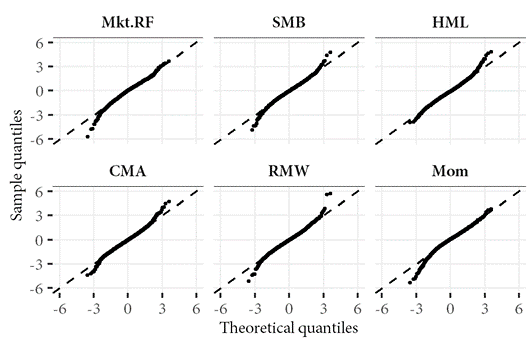
\includegraphics[width = 9cm]{graphics/qq_norm.png}
    \caption{Normal}
  \end{subfigure}
  \\
  \begin{subfigure}{9cm}
    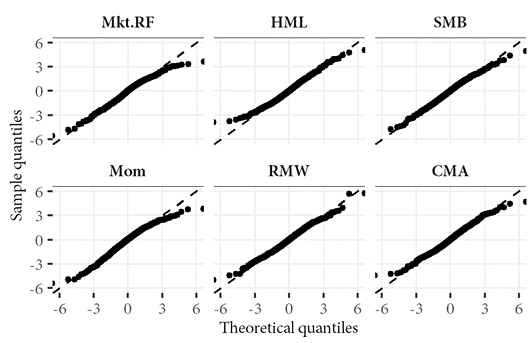
\includegraphics[width = 9cm]{graphics/qq_std.png}
    \caption{Symmetric \emph{t}}
  \end{subfigure}
  \\
  \begin{subfigure}{9cm}
    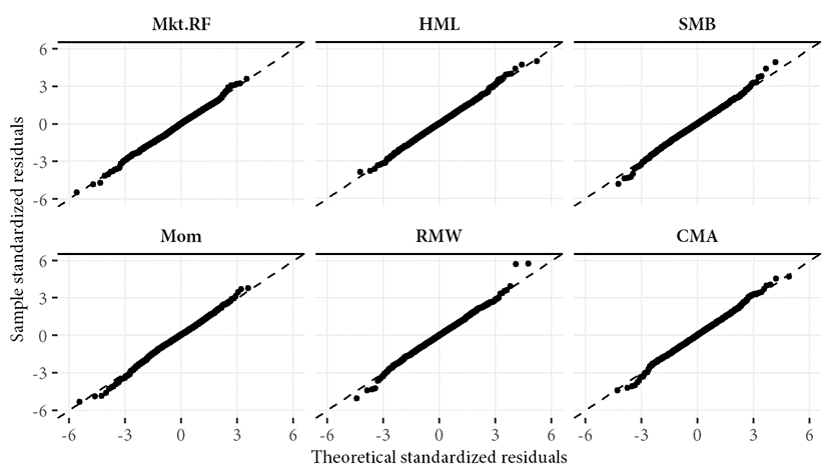
\includegraphics[width = 9cm]{graphics/qq_ghst.png}
    \caption{Skewed \emph{t}}
  \end{subfigure}
  \caption{QQ plots of standardized residuals}
  \begin{longcaption}
    Standardized residuals from the best (lowest BIC) ARMA-GARCH model specifications, with normal, symmetric \emph{t} and skewed \emph{t} innovations. Data from the theoretical distribution should line up on the dashed line. Based on weekly data 1963--2016.
  \end{longcaption}
  \label{fig:garch_qq}
\end{figure}

% In the variance equation, all factors exhibit high $\alpha$ and $\beta$ leading to a high variance persistence, between 0.96 and 0.99. Generally, variance persistence, which is related to volatility clustering, tends to be high in financial return series. [WHAT DOES IT MEAN WHY DO I CARE] We note that the zero-cost factor portfolios are no exception. The HML factor has a higher $\alpha$ estimate, indicating that shocks of equal size translate into slightly stronger volatility for HML than for RMW and CMA. RMW, on the other hand, has both the lowest $\alpha$ estimate and the highest $\beta$ estimate, indicating higher persistence and lower sensitivity of volatility to shocks.

% We note that the Mkt.RF factor is, according to our model selection procedure, best fitted by a ARMA(0, 0) mean equation, indicating no predictive power of 1-week lagged returns. Also, in the variance equation, we note that the relatively low $\alpha = 0.037$ sensitivity to shocks is increased considerably by $\eta = 0.181$ in the case of a \emph{negative} shock. Furthermore, the Mom factor stands out with a much higher estimate of $\alpha$ (0.186) than any of the other series (all around 0.10) and a lower $\beta$ (0.793). This means that volatility in the momentum factor is more sensitive than other factor strategies to return shocks and less predictable by past volatility alone. We also note that the Mkt.RF and Mom factors exhibit relatively higher unconditional volatilities (of 0.022 and 0.018) than do other factors (around 0.010).

Many of the estimates of $\gamma_i$, the skewness of the skewed \emph{t} GARCH innovation process, are statistically insignificant. This is also the case for the degree of freedom estimates, $\nu$ for the SMB and Mom models. Although these parameters are not significantly estimated, we believe that including them is essential, as QQ-plots indicate misspecification for the models with normal and symmetric \emph{t} innovations.

% subsection univariate_modeling_of_returns (end)
 % arma garch

%!TEX root = ../../main.tex

\subsection{Multivariate dependence} % (fold)

In this subsection, we demonstrate that the standardized residuals $z_{i,t}$ in our chosen ARMA-GARCH models display both asymmetric and time-varying dependence, shown by threshold and rolling correlations. ARMA-GARCH filtering has little effect on the (time-varying) correlations between factors. However, the use of the skewed \emph{t} distribution does remove a degree of asymmetry in the dependence. These patterns in multivariate dependence are the motivating reasons for a copula model, as they suggest that factor returns are not independent of each other after filtering for univariate effects, and that this dependence is not well-approximated by a normal model.\footnote{A visual comparison of dependence measures on returns compared to standardized residuals can be found in~\autoref{app:supplementary}.}

% XXX Här finns en liten karamell att suga på; gammal text nedan

% , measured by threshold correlations, and time-varying correlations, measured by rolling correlations, features we will attempt to model in the copula model. In the context of modeling, we are interested in the standardized residuals, rather than the returns themselves, as they are filtered of the variance dynamics present in the returns themselves~\autocite{ChristoffersenLanglois2013}.\footnote{The visual patterns for both threshold and rolling correlations are quite similar between returns and standardized residuals; results are available in the appendix.}

\subsubsection{Threshold correlations}

Threshold (or exceedance) correlations have previously been used to highlight the asymmetric dependence structure of i.a. country equity indices~\autocite{LonginSolnik2001}, portfolios by industry, size, value and momentum~\autocite{AngChen2002} and factor strategies~\autocite{ChristoffersenLanglois2013}. The following analysis is still new as it adds the investment (CMA) and profitability (RMW) factors. We follow~\textcite{ChristoffersenLanglois2013} definition of threshold correlation:
\begin{align}
\label{eq:th_corr}
    ThCorr(r_i, r_j) = 
    \begin{cases} 
        Corr\Big(r_i, r_j \,|\, r_i < F_i^{-1}(p), r_j < F_j^{-1}(p)\Big)  & \text{for } p < 0.5 \\
        Corr\Big(r_i, r_j \,|\, r_i \geq F_i^{-1}(p), r_j \geq F_j^{-1}(p)\Big)  & \text{for } p \geq 0.5
    \end{cases}
\end{align}
% XXX Be consistent with percentile and quantile
where $F_i^{-1}(p)$ is the empirical quantile of $r_i$ at percentile $p$. Threshold correlations thus reflect how series correlate when both are simulataneously realizing in their respective tails. This subsetting of data is illustrated in \autoref{fig:illustrate_threshold}. In the left hand plots, we see the scatter of ARMA-GARCH residuals of Mkt.RF and HML respectively, and how the threshold $p$, found on the $x$-axis of the right hand plot, determines the subset of data that is included in the correlation calculation. We note that the unconditional (standard) correlation, given by the dashed line in the right hand plot, is clearly negative, while threshold correlations in the first and third quadrants are significantly more positive, which shows that not taking threshold correlations into account provides a vaguer picture of the dependence structure when both factor series realize in the tails.

\begin{figure}[H]
  \centering
  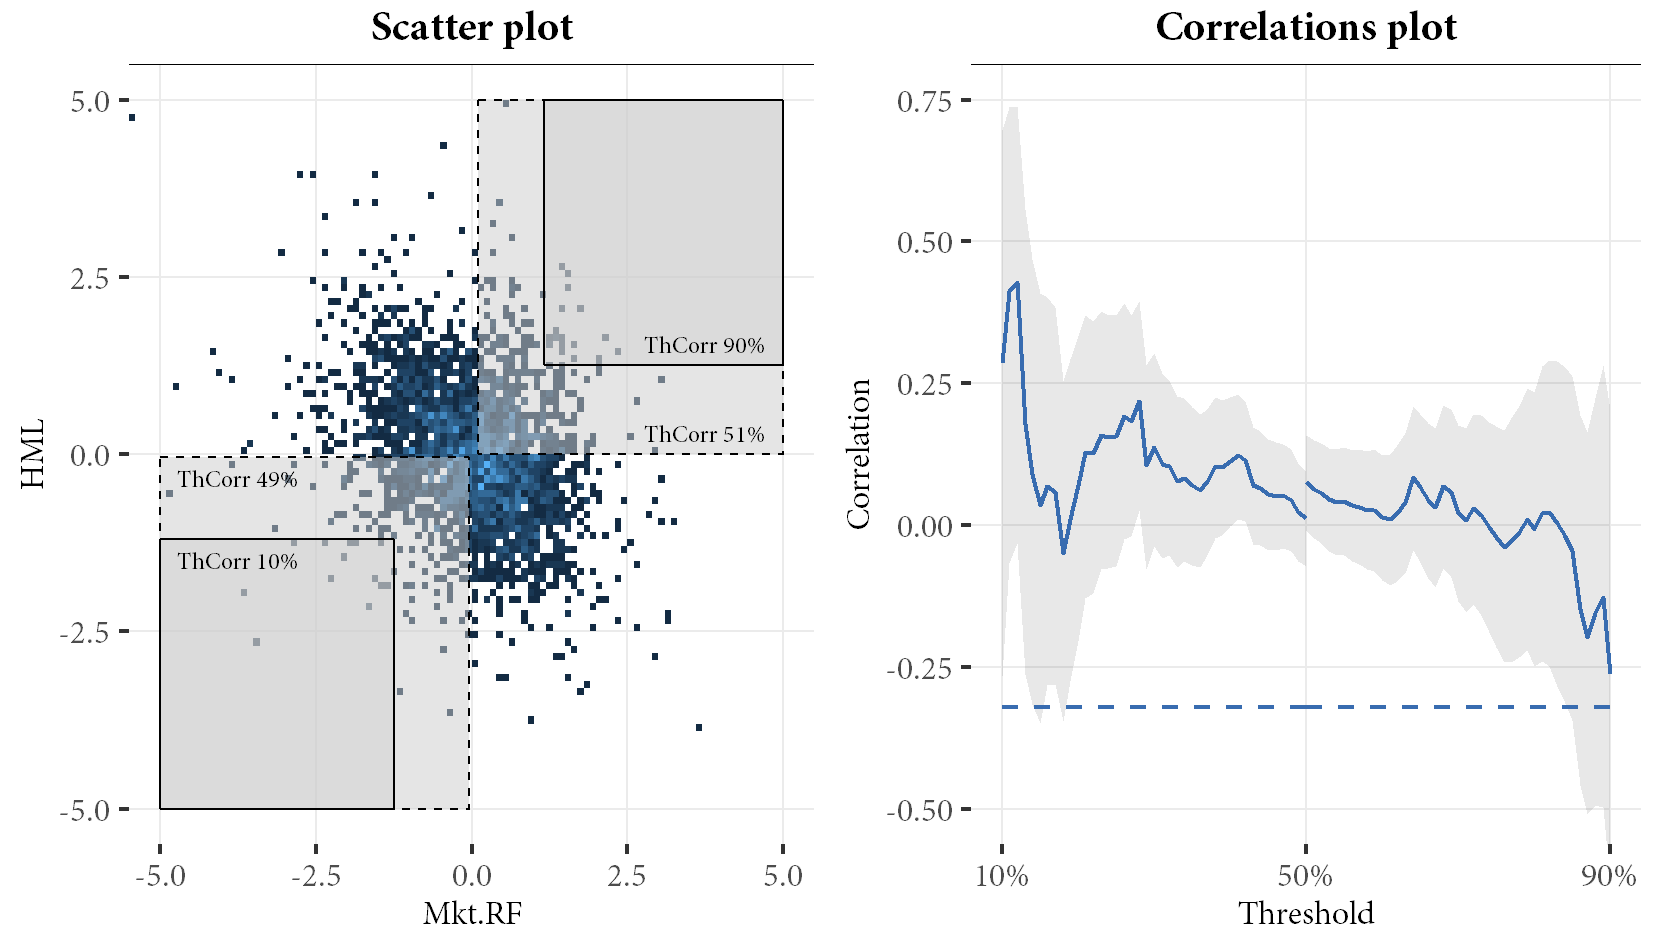
\includegraphics[scale=1]{graphics/threshold_explain_res.png}
  \footnotesize
  \caption{Illustration of threshold correlations}
  \begin{longcaption}
    ARMA-GARCH residuals from the Mkt.RF--HML asset pair. 95\% shaded confidence bounds. The unconditional correlation is given by the dashed line. Based on weekly data 1963--2016.
  \end{longcaption}
  \label{fig:illustrate_threshold}
\end{figure}

We now plot threshold correlations without the adjacent scatter graph. \autoref{fig:threshold1} displays threshold correlations for HML, CMA and RMW against each other as well as against the the other factors Mkt.RF, SMB and Mom. We note that for most asset pairs, the threshold correlation is significantly different from the unconditional correlation coefficient given by the dashed line.

We also note that there is asymmetry around the median for some factor pairs, including the Mom--CMA, RMW--HML, RMW--CMA, and to a lesser extent Mkt.RF--RMW, asset pairs. For example, in the Mom-CMA asset pair, the threshold correlation jumps up for the first percentile below the median, indicating that the correlation is higher when both realize below the median than when both realize above the median. This type of asymmetric property, where downside (below the median) correlation is higher than upside correlation is unwanted, as it reflects a poorer diversification in bad times. The opposite type of asymmetry can be seen for the HML--RMW and CMA--RMW asset pairs; When these factors simultaneously realize above the median, they are significantly more correlated. This pattern presents no diversification problem.

Although estimated with substantial uncertainty, the threshold correlations do not seem to be constant as the threshold $p$ approaches either zero or one. For example, the Mkt.RF--HML asset pair seems to have a downward pattern, where correlations are the most positive in the lowest percentiles of residuals and the most negative in the highest percentiles of residuals. In fact, this pattern is unwanted from a diversification perspective, as series tend to coincide more in extreme negative events. 

The CMA--HML pair stands out from the other factors. The pair exhibits an unusually high correlation in excess of $0.60$ with a virtually flat threshold pattern. HML and CMA are also generally similar to each other in their respective threshold patterns to other factors -- most notably in the HML/CMA--RMW pairs. They differ in the presence of a break around the median in Mom--CMA not present in Mom--HML.

RMW is the only factor to be virtually uncorrelated with Mkt.RF in the lower tails, suggesting that it is a good diversifier in market downturns. This is very different from the pattern of higher threshold correlations as $p$ approaches zero for e.g. Mkt.RF--HML. For Mkt.RF--HML, the higher lower tail correlation could be related to the industry over-capacity hypothesis discussed in~\autoref{sec:literature}, i.e. that value firms are particularly sensitive to market downturns due to unproductive capital.

While the patterns in threshold correlations are interesting, we are careful not to draw conclusions regarding diversification benefit based on solitary threshold correlation graphs -- what is interesting is the total pattern, and our key point is that there seems to be tail dependence that should not be ignored in the copula specification.

\begin{figure}[p]
  \centering
  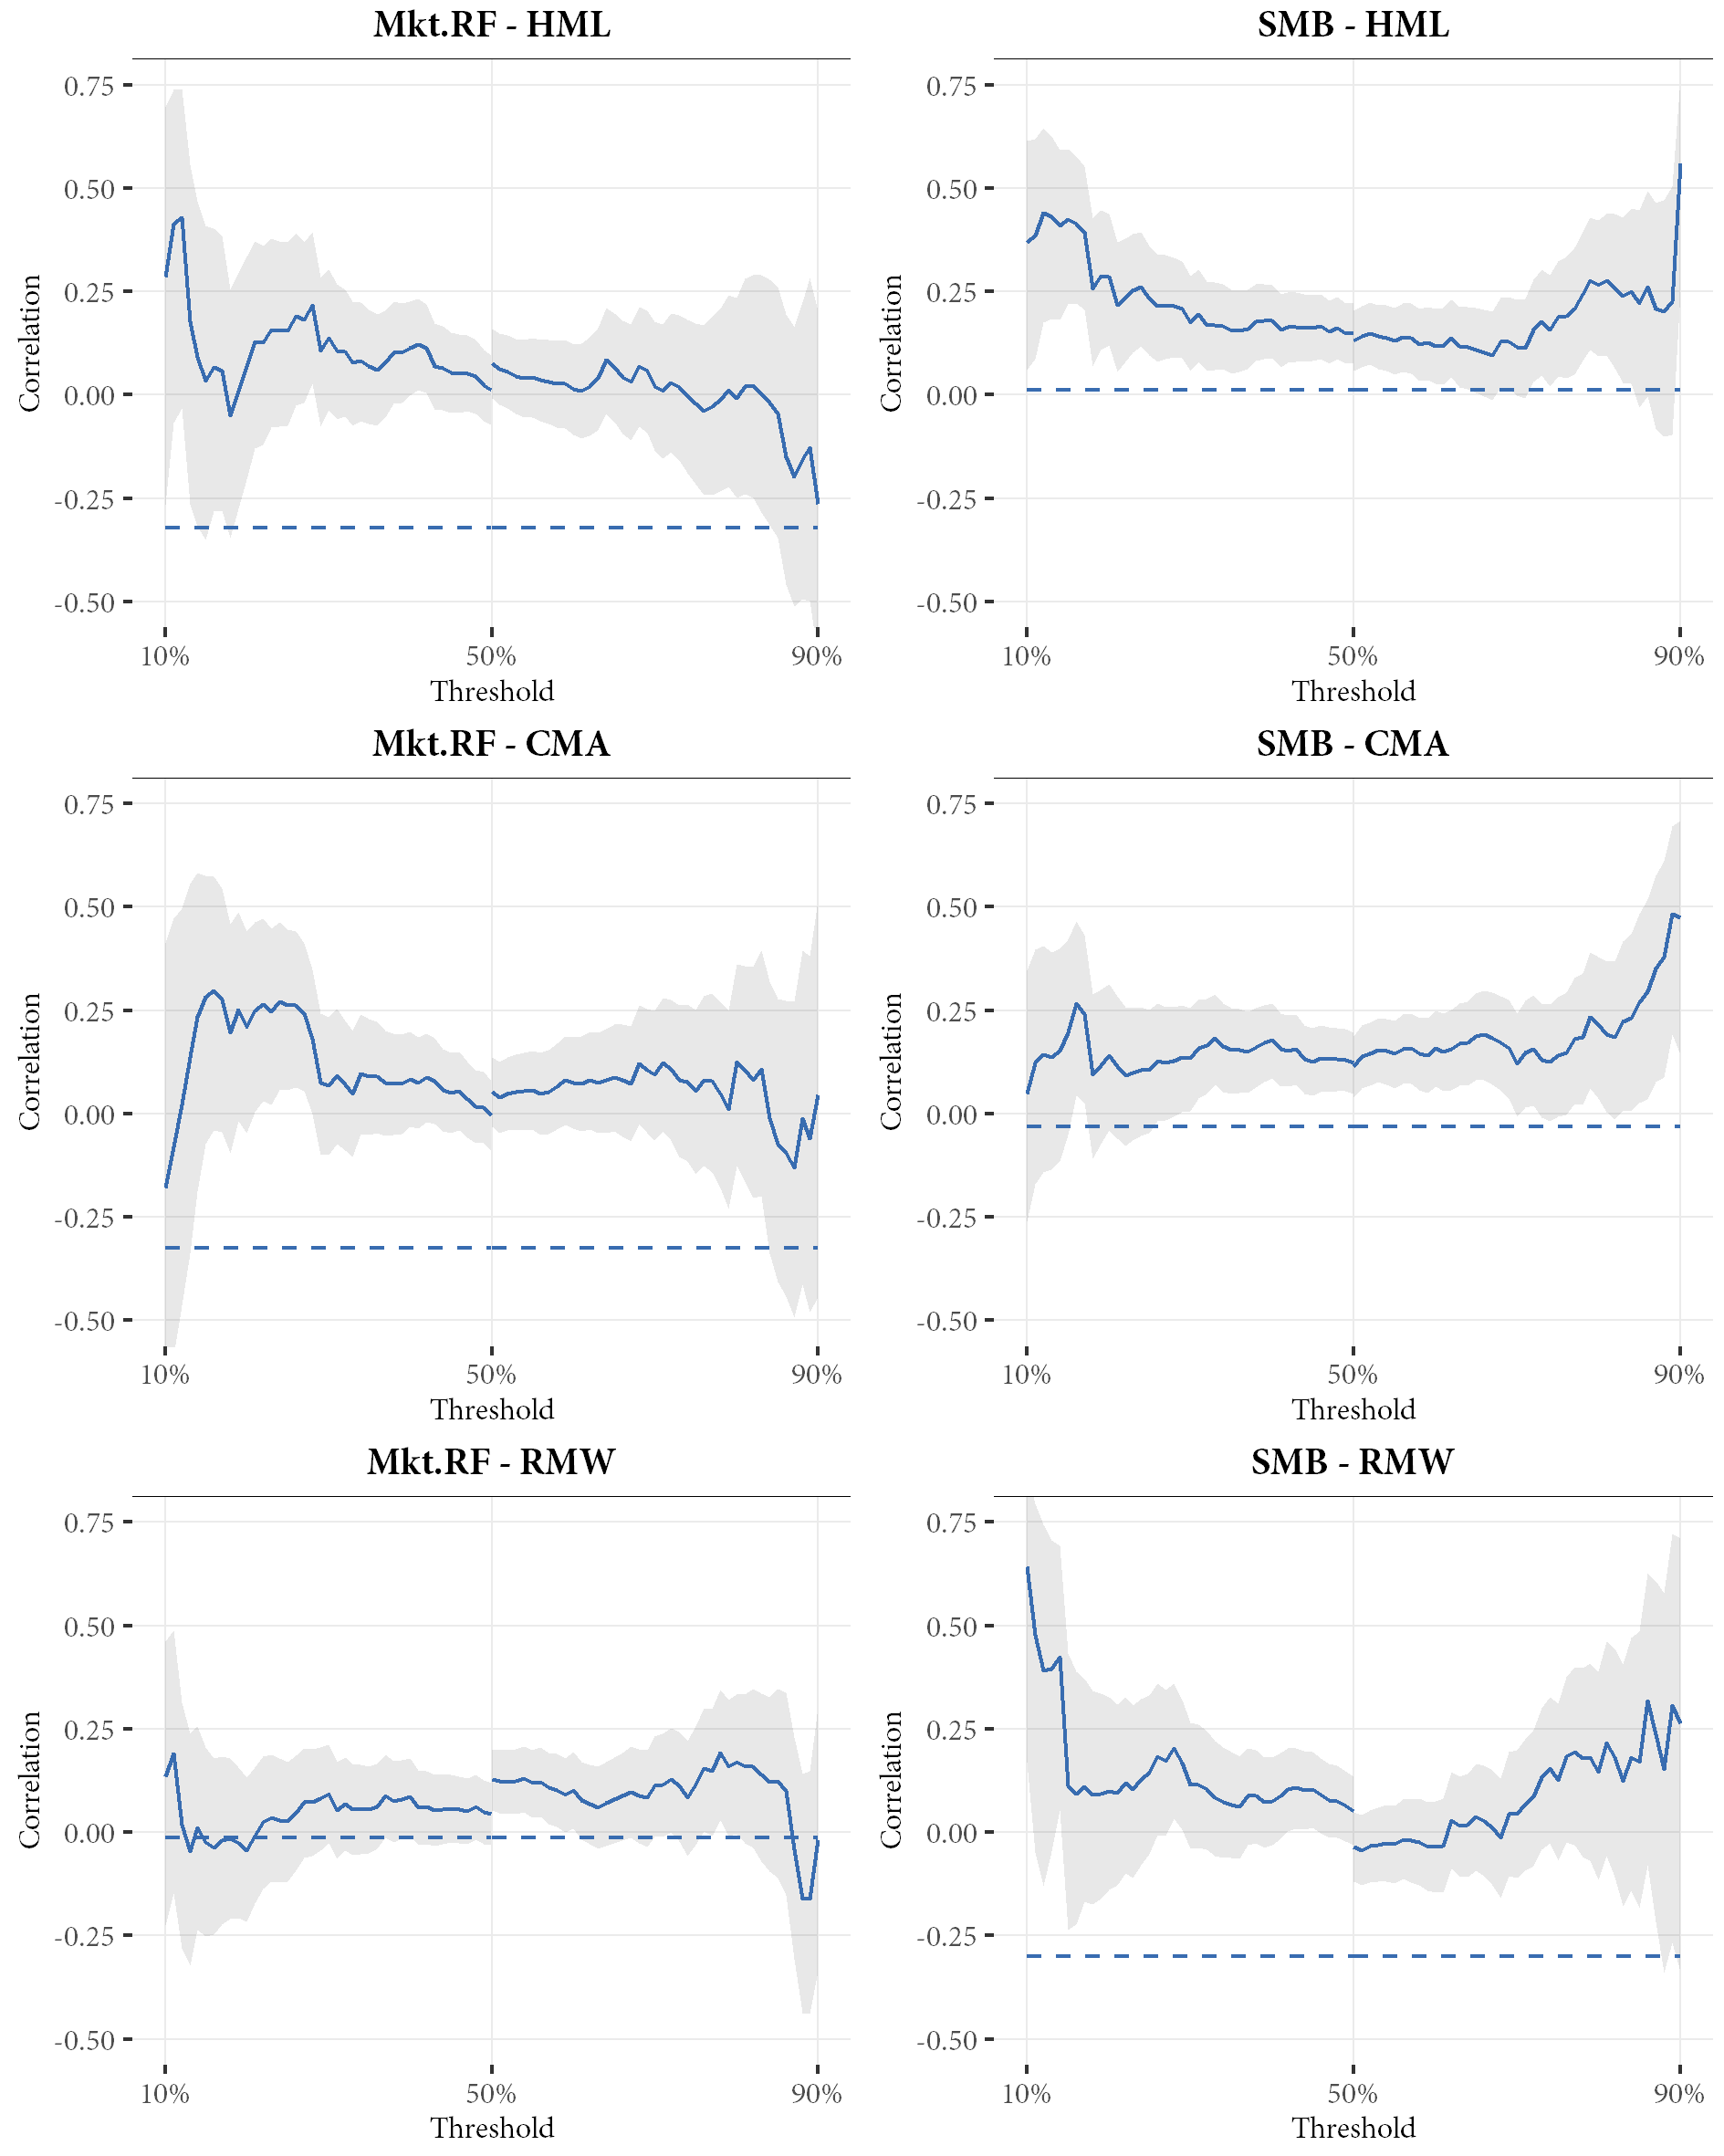
\includegraphics[scale=1]{graphics/threshold1.png}
  \footnotesize
  \caption{Threshold correlations of ARMA-GARCH standardized residuals}

  \begin{longcaption}
    The formula for threshold correlations for a threshold $p$ is given in~\autoref{eq:th_corr}. 95\% shaded confidence bounds, taking the model as given. The unconditional correlation is given by the dashed line. Based on weekly data 1963--2016.
  \end{longcaption}
  \label{fig:threshold1}
\end{figure}
\begin{figure}[p]
  \ContinuedFloat
  \centering
  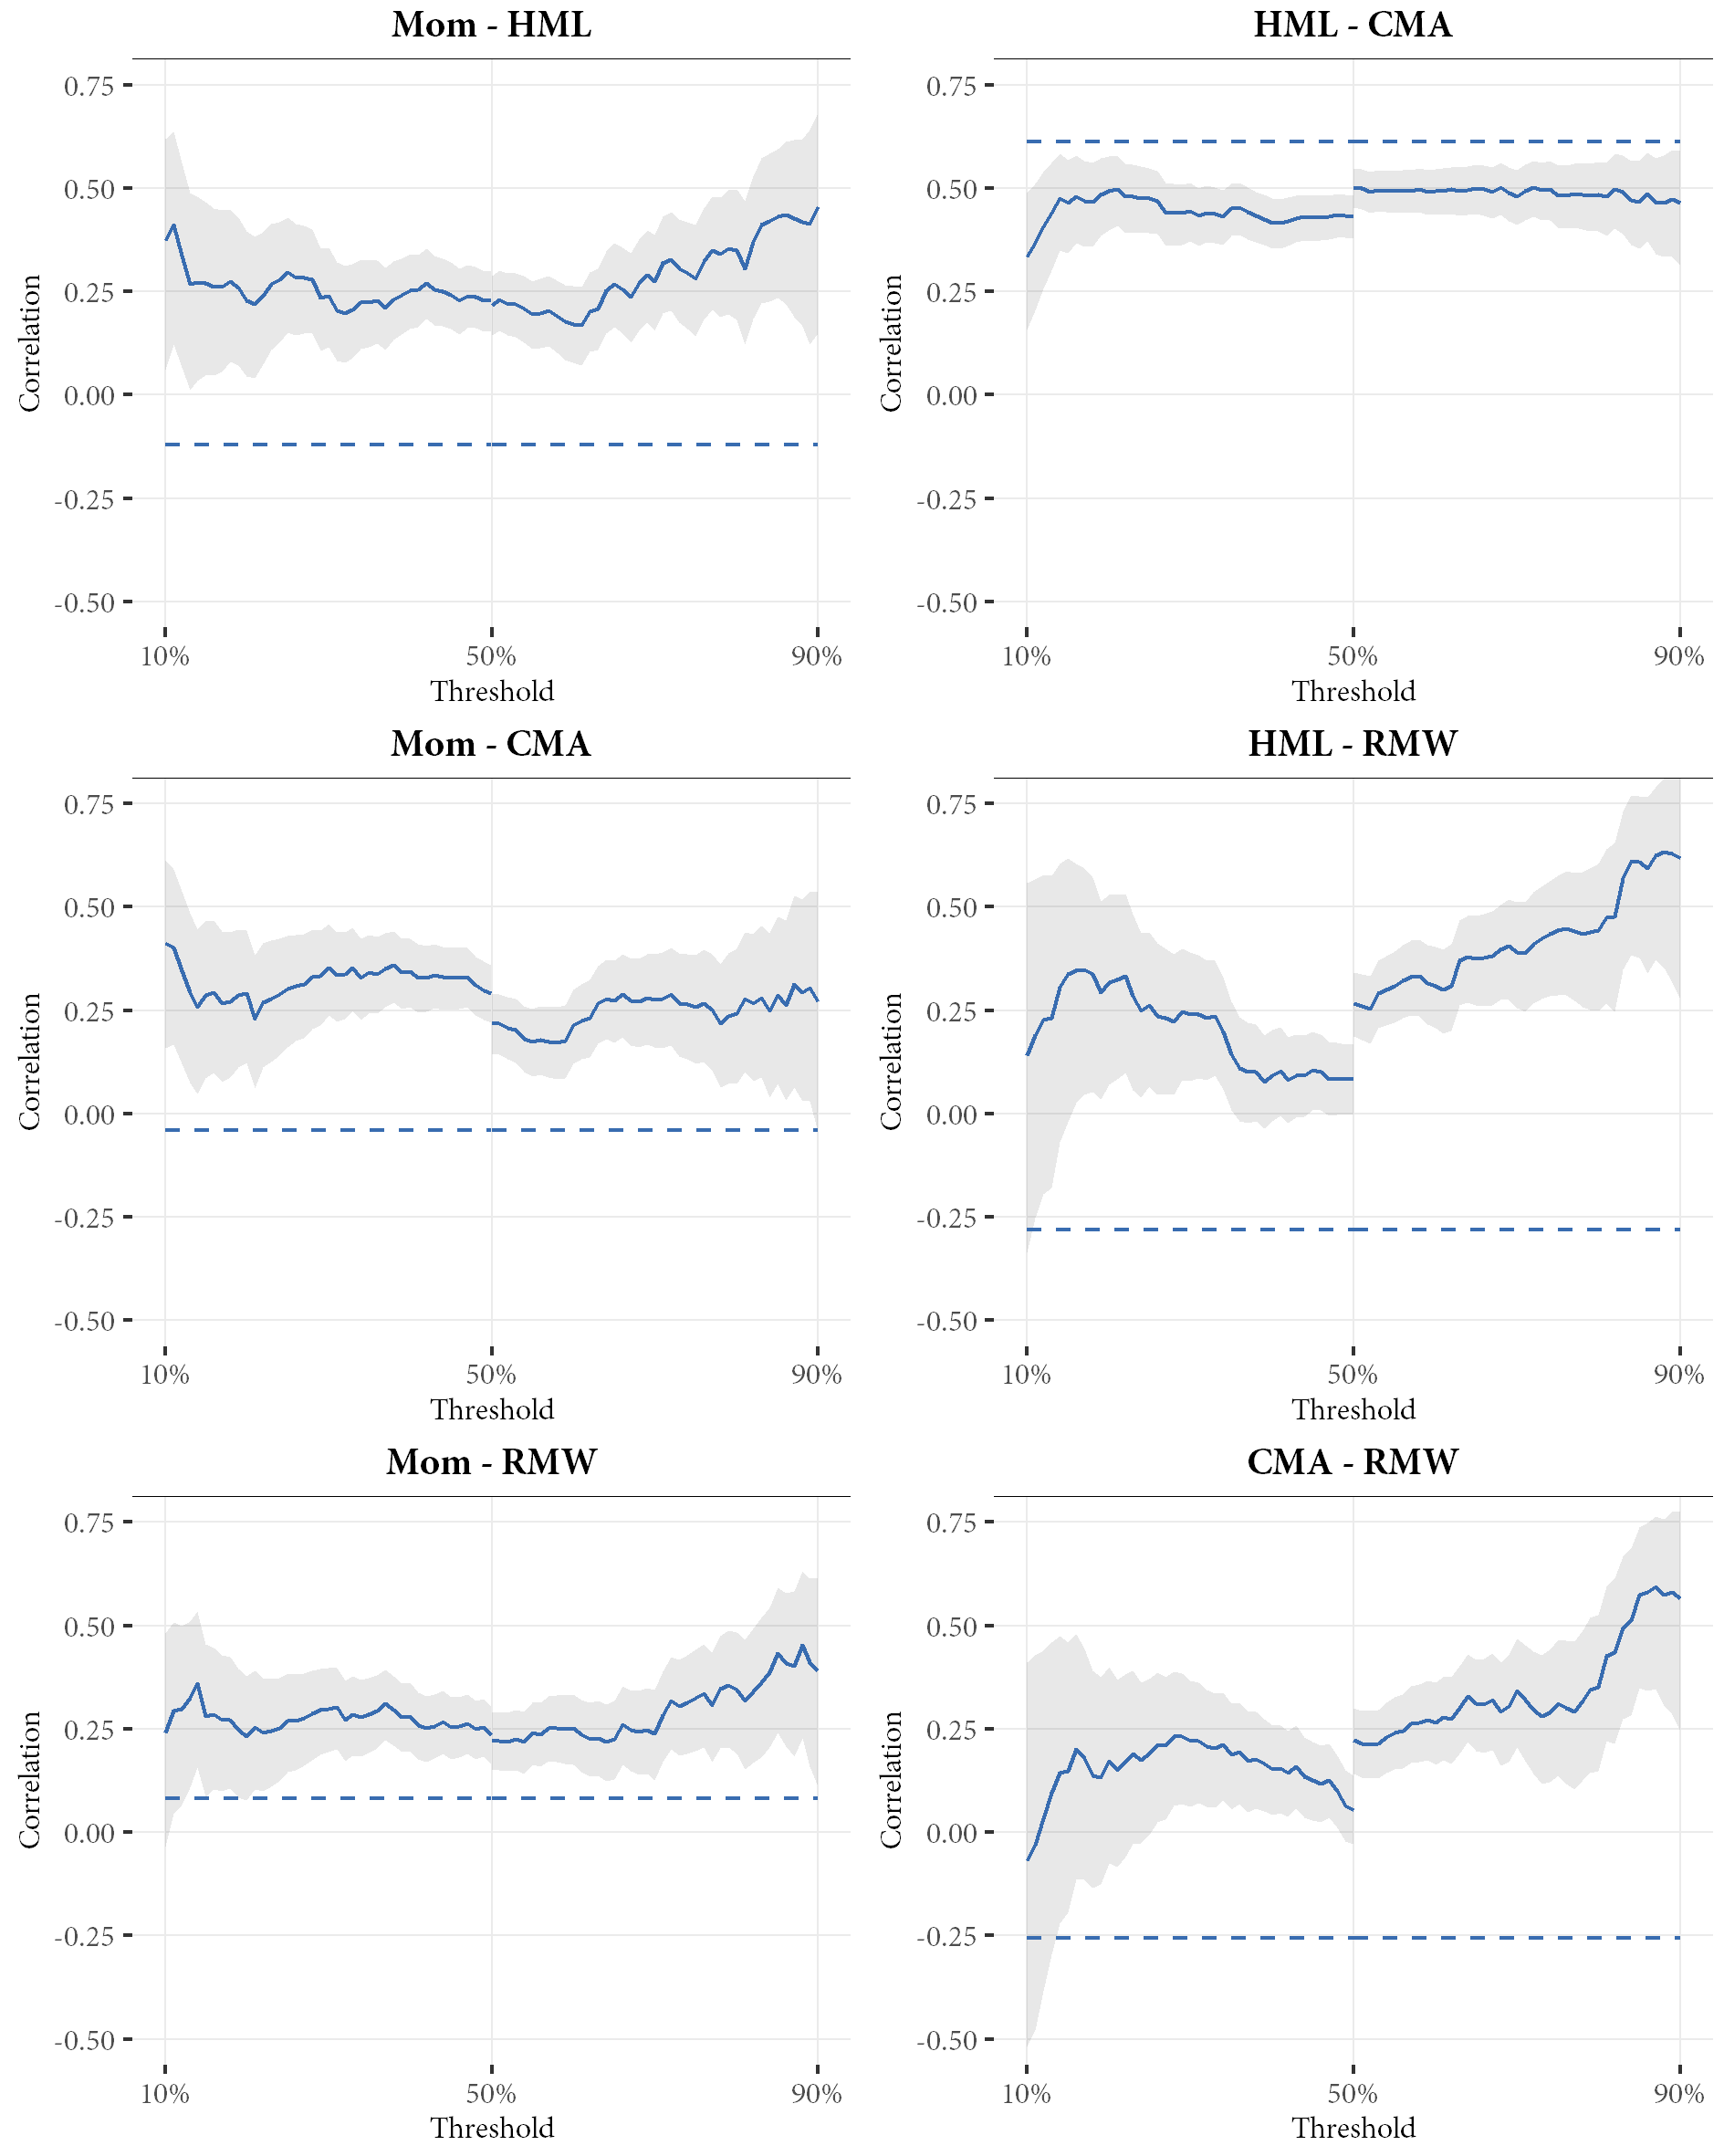
\includegraphics[scale=1]{graphics/threshold2.png}
  \footnotesize
  \caption{Threshold correlations of ARMA-GARCH standardized residuals (cont.)}
\end{figure}

\subsubsection{Rolling correlations}

We compute rolling 52-week correlations between the factors on standardized residuals of our ARMA-GARCH models, according to the formula: 
\begin{align}
    RCorr(r_{i, t}, r_{j, t})_t^{52} = \frac{\sum^{t}_{t-51}(r_{i, t} - \bar{r}_i)(r_{j,t} - \bar{r}_j)}{\sqrt{\sum^{t}_{t-51} (r_{i,t} - \bar{r}_i)^2} \sqrt{\sum^{t}_{t-51} (r_{j,t} - \bar{r}_j)^2}}
\end{align}
where $r_i$, $r_j$ are the different pairs of the factor strategies' ARMA-GARCH residuals.\footnote{Rolling correlations for the returns themselves are available in the \autoref{app:supplementary}.} Results are presented in ~\autoref{fig:rolling1}.
% plots
\begin{figure}[!p]
  \centering
  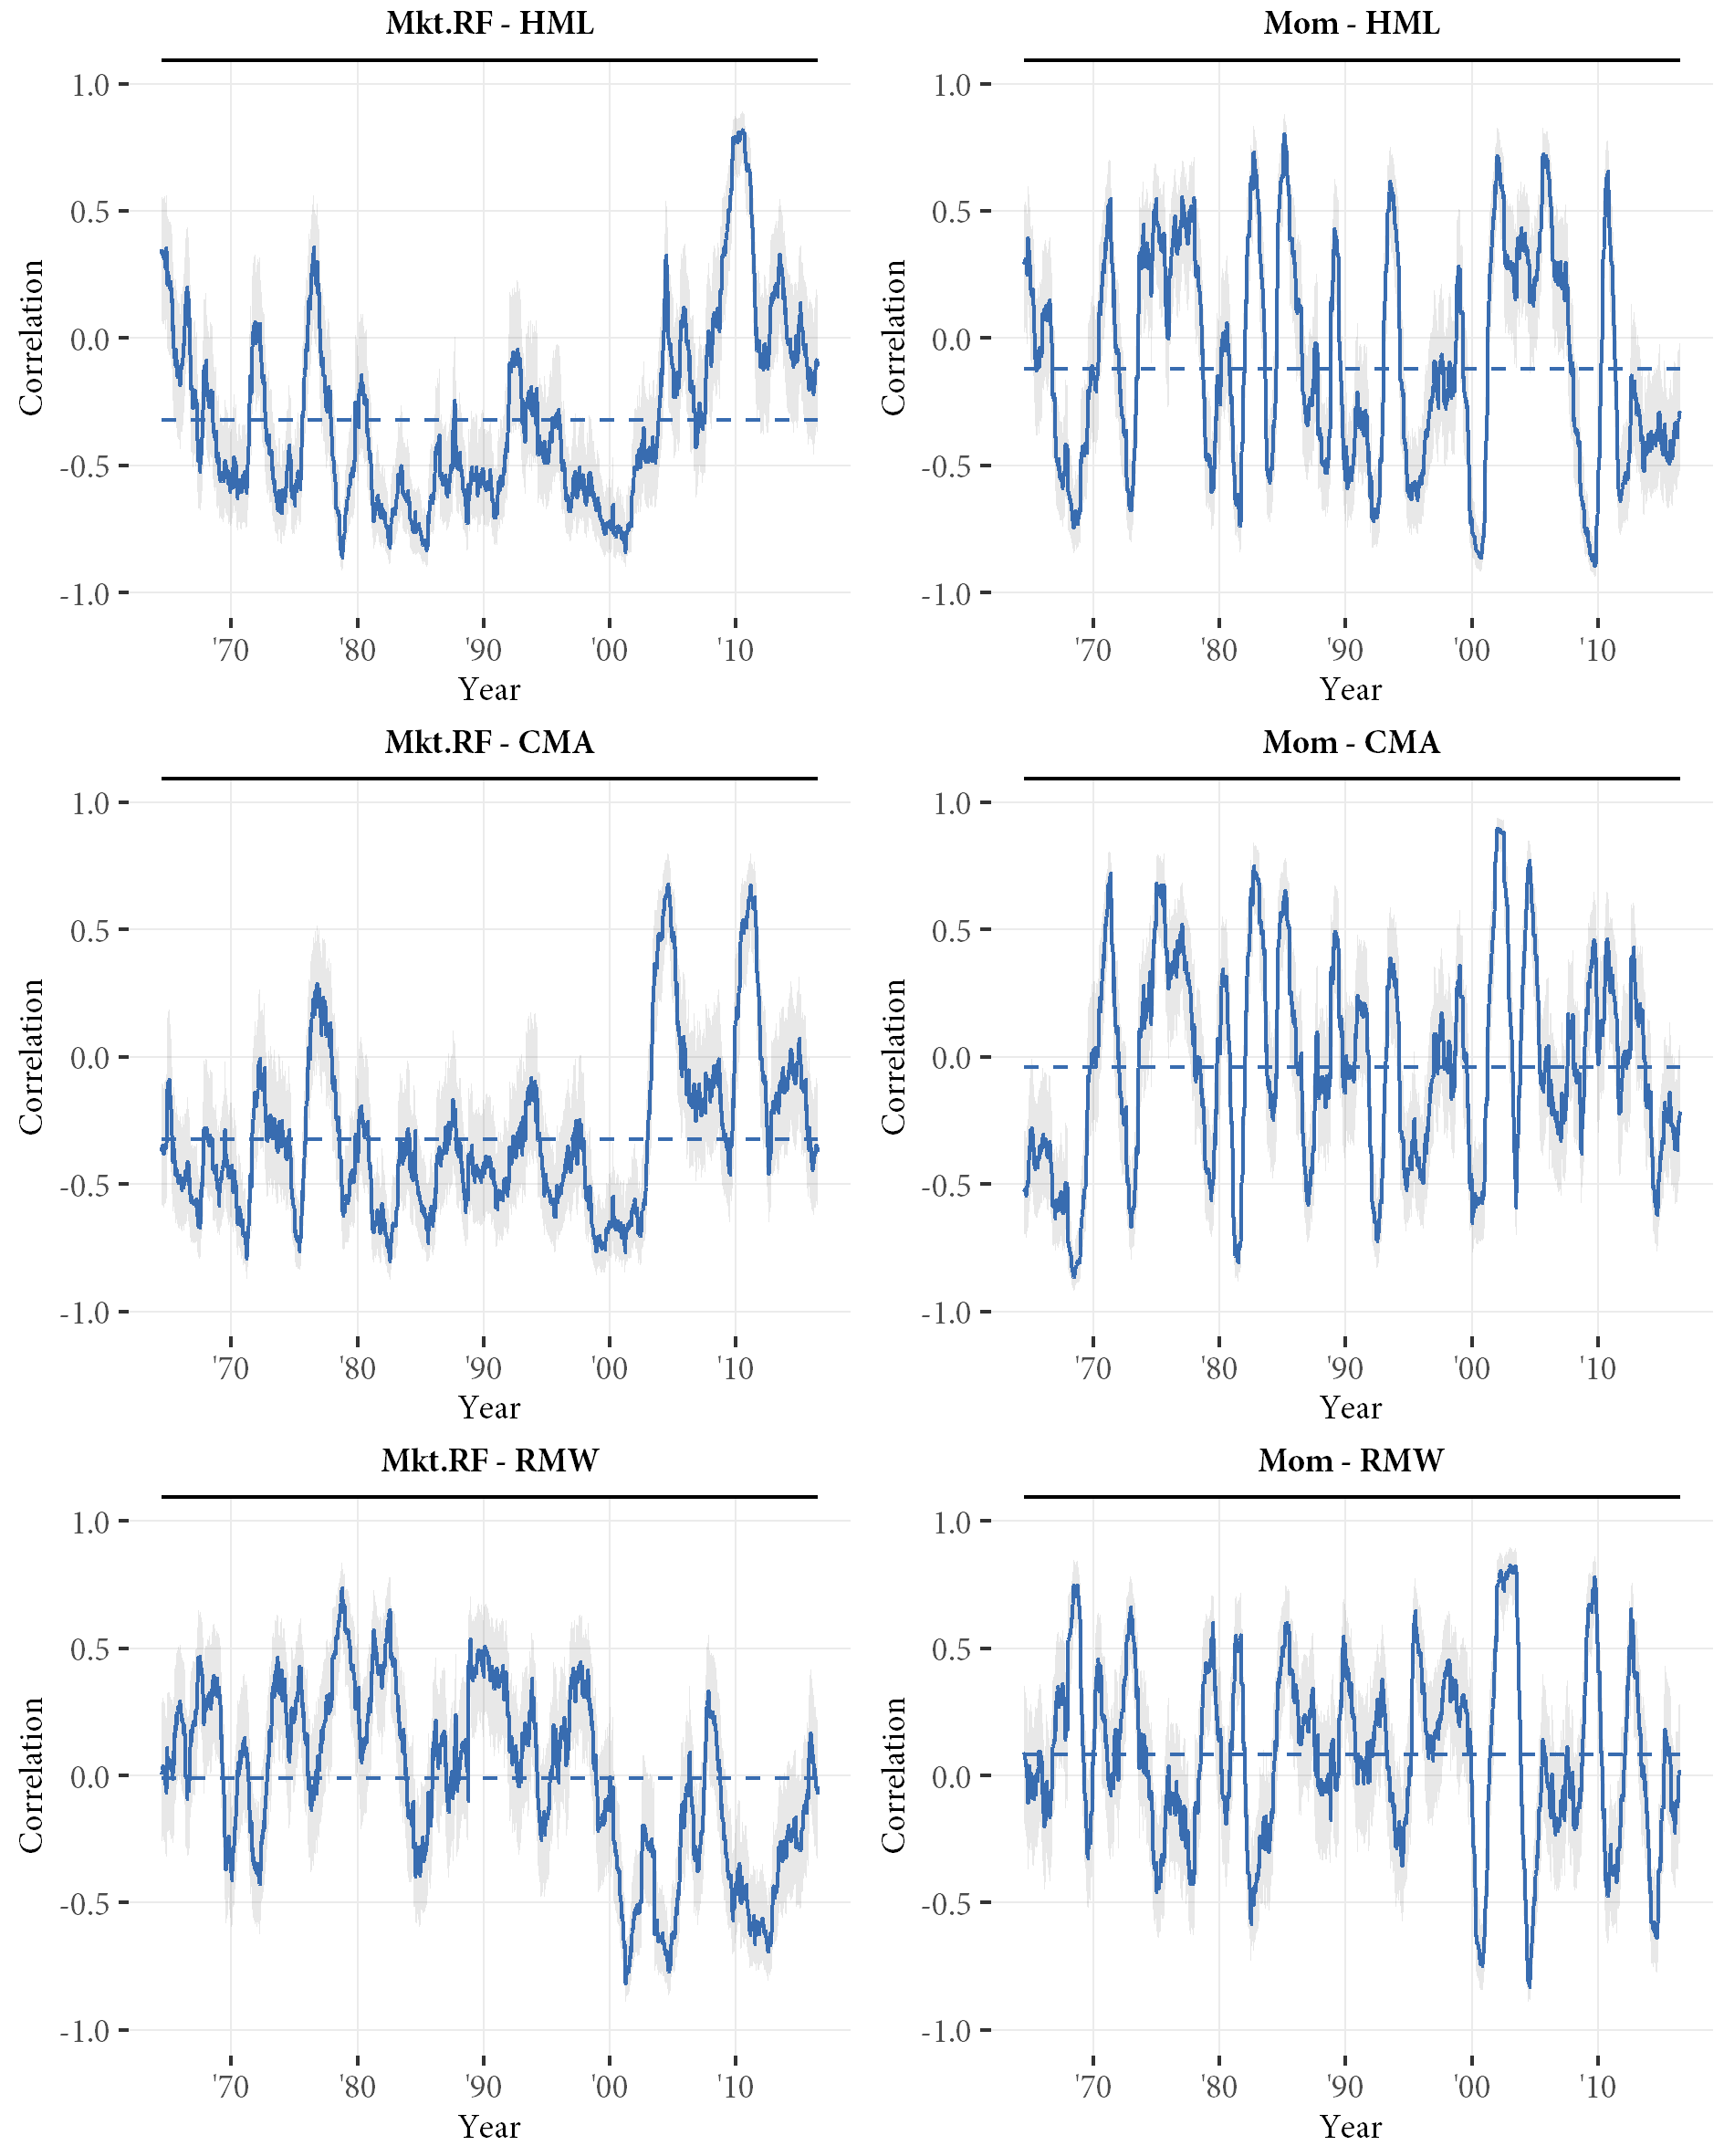
\includegraphics[scale=1]{graphics/rolling1.png}
  \footnotesize
  \caption{Rolling correlations of ARMA-GARCH standardized residuals}
  \begin{longcaption}
    95\% shaded confidence bounds, taking the model as given. The unconditional correlation is given by the dashed line. Based on weekly data 1963--2016.
  \end{longcaption}
  \label{fig:rolling1}
\end{figure}
\begin{figure}[!p]
  \ContinuedFloat
  \centering
  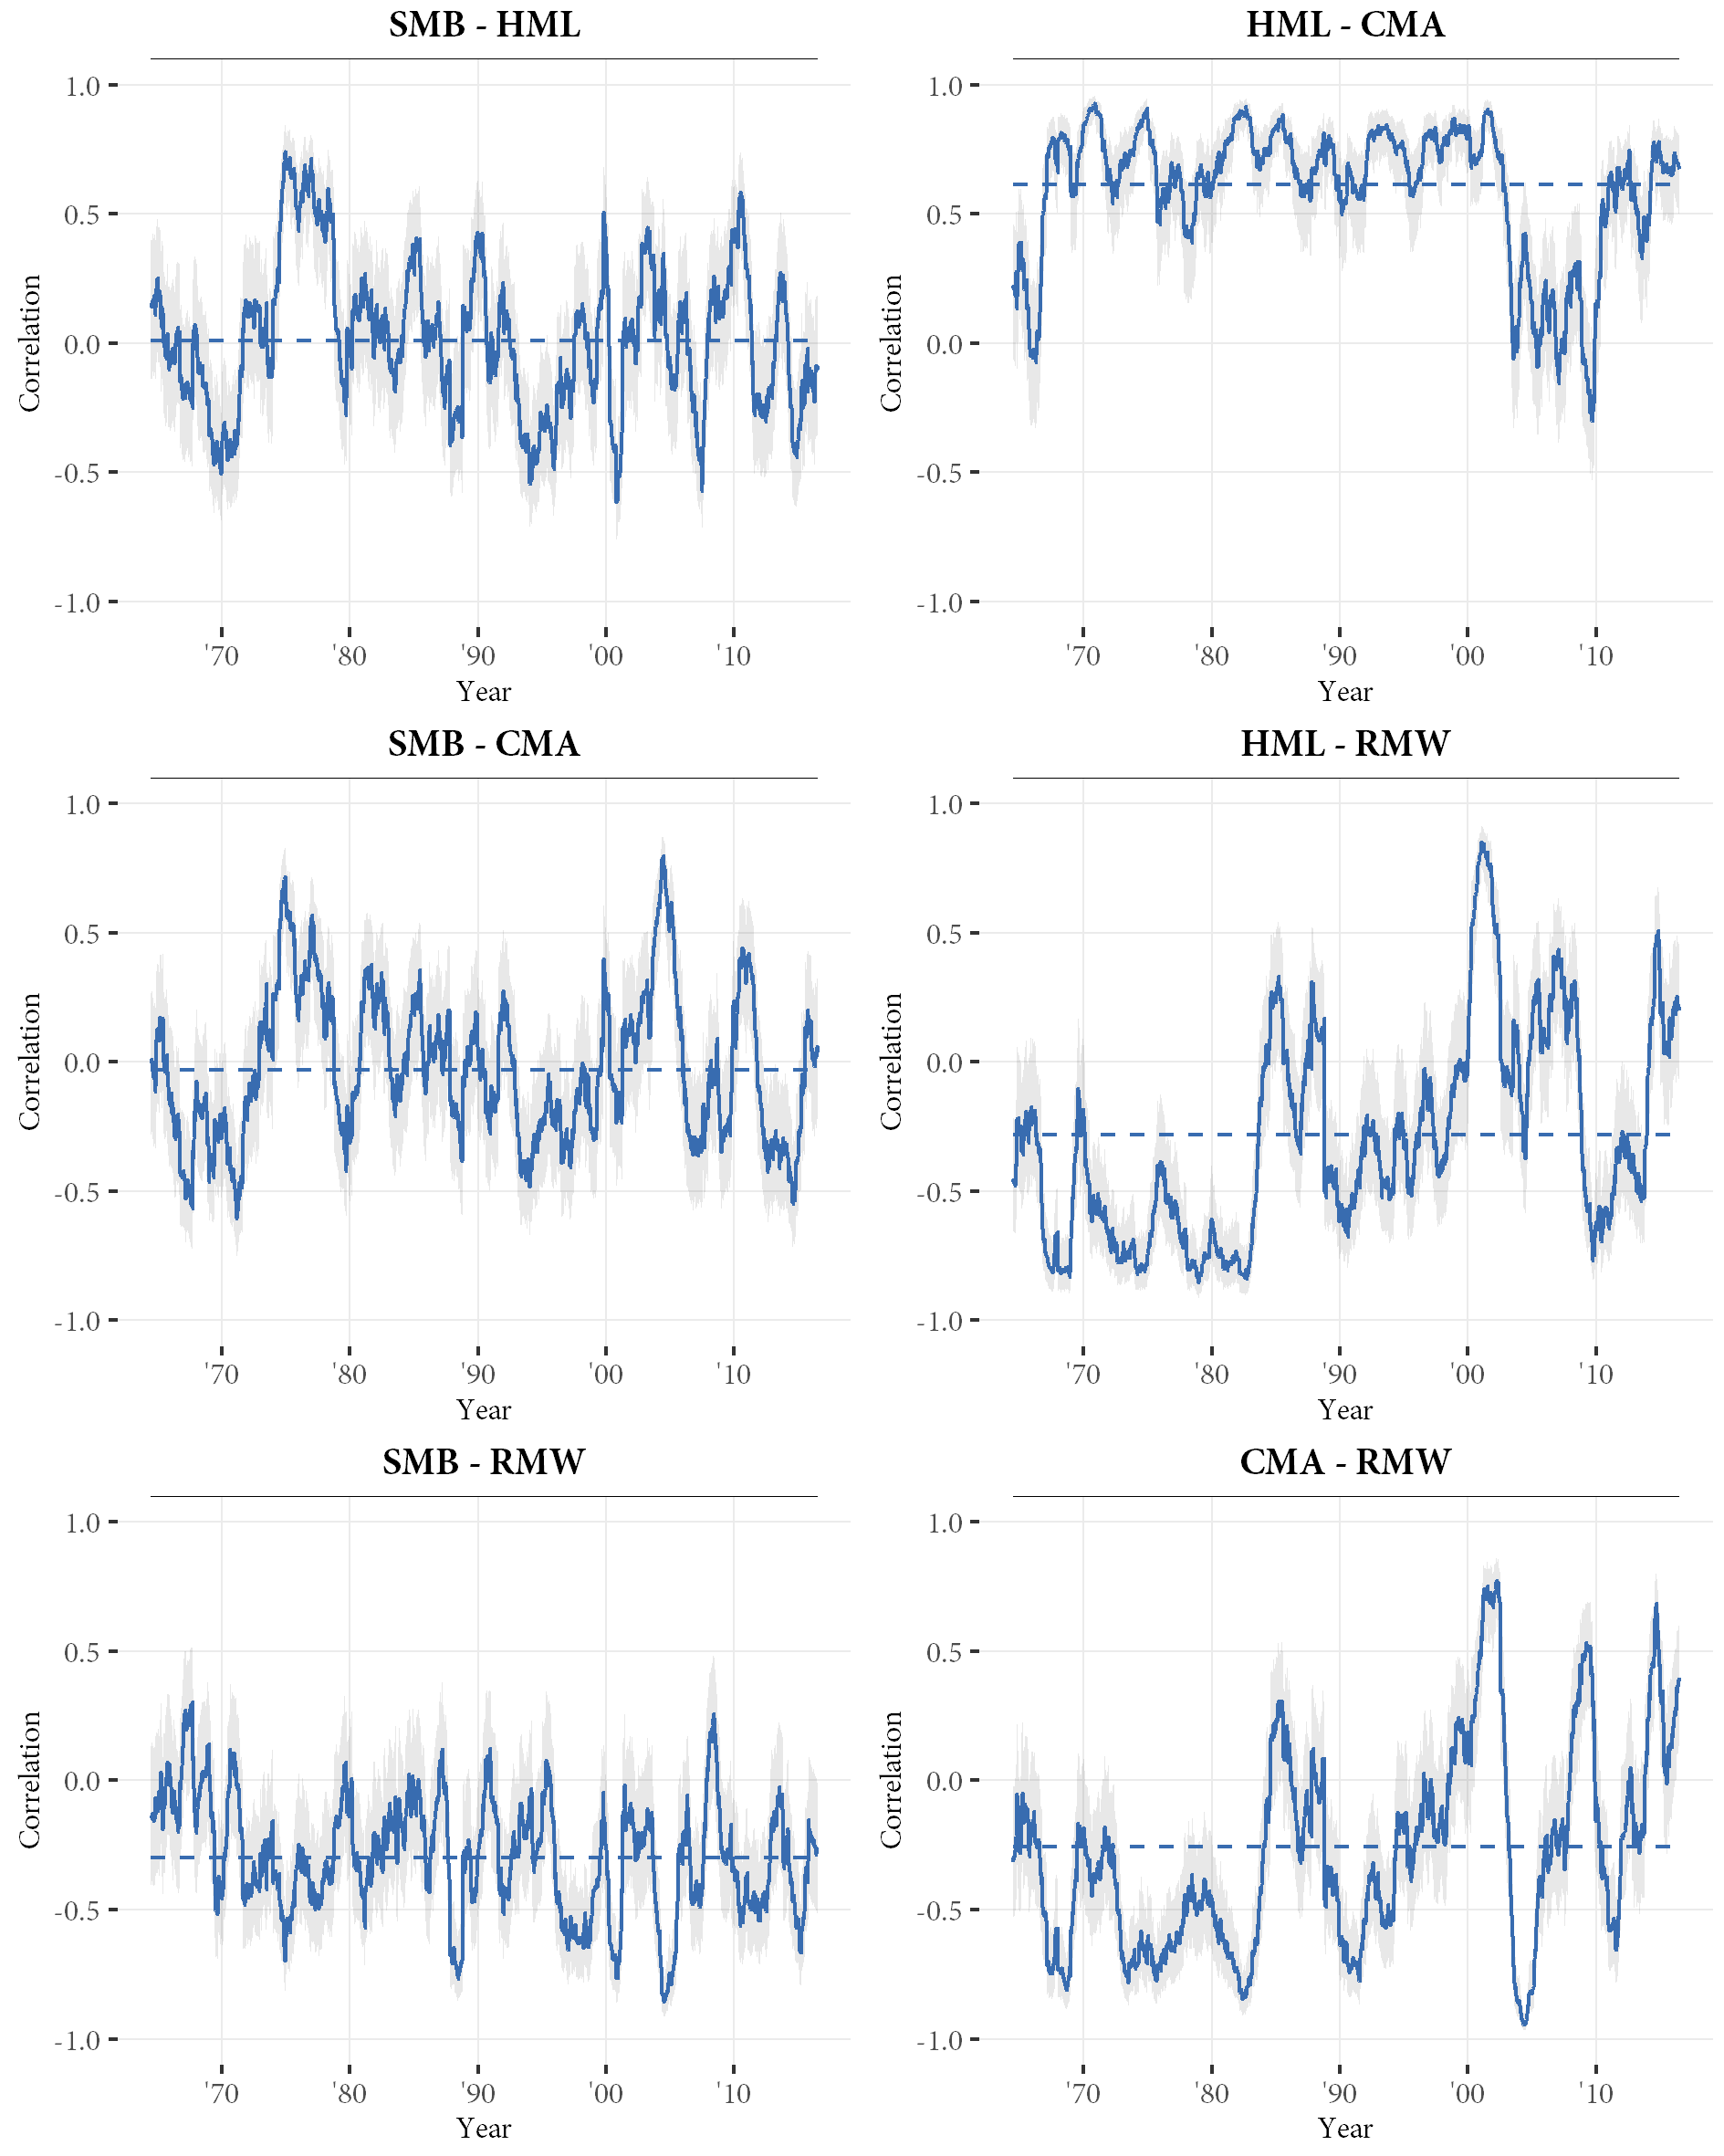
\includegraphics[scale=1]{graphics/rolling2.png}  
  \footnotesize
  \caption{Rolling correlations of ARMA-GARCH standardized residuals (cont.)}
\end{figure}
% talk
First, we note that for most factor pairs, the rolling 52-week correlations are time-varying, and indeed appear to swing wildly. The unconditional correlation of Mkt--HML is negative in the studied time period, but rolling correlations range between -0.75 and 0.75. Also of note is the momentum factor's rapid shifts between positive and negative correlations to the other factors. 

% Value and profitability in crisis times?
Second, by visual inspection, we see no obvious trend in the correlations between factor pairs. There are, however, notable patterns around the 2000--2001 bubble period -- here, the correlations of HML--RMW, CMA--RMW and Mkt--CMA appear to jump sharply. This is an indication that diversification benefits may be time-varying. Another interesting pattern is that the correlations of Mkt--RMW went down sharply around this period -- in line with the idea that profitable firms are stronger and better at weathering crises than the average firm~\autocite{NovyMarx2013}. The 2000--2001 period may represent a structural break in the dependency patterns between factors, with the appearance of persistent differences before and after -- however, there is not enough post-2000 data to support such a conclusion, yet.

Third, the HML--CMA factor pair again stands out as different from other factor pairs. The unconditional correlation is much closer to the rolling estimates than for other factor pairs, with a dip in the 2000--2010 period that appears to have gone away. Clearly, the HML--CMA pair is the most strongly correlated factor pair, even when considering subperiods of the data.

Our key takeaway from the rolling correlations is that there seems to be persistency in the time-variation in correlations. This could be incorporated in the copula specification, which then needs to have a time-varying correlation matrix, $\Psi_t$.

% \subsubsection{Takeaways from Analysis of Multivariate Dependence}

% Univariate residuals appear to be white noise series with no remaining autocorrelation or volatility clustering. However, there is important dependence between residuals of different strategies. First, threshold correlations show that there is tail dependence -- in times when factor pairs simultaneously realize in their best and worst percentiles, correlations are significantly different from the unconditional correlations. In fact, threshold correlations are substantially higher than the unconditional correlations, which indicates that diversification benefits are smaller than expected when factors simultaneously experience bad (or good) times. Second, rolling correlations show that correlations between series are highly time-varying and seem to exhibit persistence. A copula model that incorporates both tail dependence and time-varying dependence is likely to improve on the description of joint returns.

% Both analyses also show that the HML-CMA asset pair is quite different from the other pairs, exhibiting a much higher and more stable dependence. Differently put, they look quite similar as opposed to any other factor pair, and the merit of including both in factor portfolios seems more unclear.

\label{sub:threshold_and_rolling_correlations_of_residuals}

% subsection threshold_and_rolling_correlations_of_residuals (end)
 % threshold and rolling

%!TEX root = ../main.tex
\subsection{Copula specification and estimation results}
Given the results of the dependence structure of residuals, we now discuss the best choice of copula model and present estimation results of the six competing copula specifications.

We have estimated constant and dynamic normal, symmetric \emph{t} and skewed \emph{t} copula models on the full dataset of uniform GARCH residuals. Results are presented in~\autoref{tab:copula_estimation}. 

First, we examine the choice between a normal, symmetric \emph{t} or skewed \emph{t} copula. We note that $\nu_c$ is clearly significant and suggests one of the Student's \emph{t} models with tail dependence over the normal model. Second, we examine the asymmetric specification and find that few of the $\gamma_c$ estimates appear significant. This indicates that the asymmetry is hard to capture, or that it is not well represented by this type of model. This is supported by the relatively small improvement in log-likelihood in going from a symmetric \emph{t} to skewed \emph{t} copula, and also by the fact that the BIC criterion prefers the symmetric \emph{t} model in the dynamic case. 

Second, we examine the choice between a constant and dynamic copula correlation matrix. There is a significant improvement in log-likelihood and BIC when moving from a constant to a dynamic copula, which suggests that time-varying dependence shown by rolling correlation is captured and improves the model's fit. We also find a high persistence of the correlation process, as $\alpha + \beta$, is close to a unit root.

In summary, we find that the dynamic symmetric \emph{t} copula is the best specification, as it has the lowest BIC, well defined parameters, and is strongly supported by the dependence pattern showcased by threshold and rolling correlation analyses. While the skewed \emph{t} copula is an interesting model, we believe that the asymmetry patterns in data are too irregular to be well captured by a copula model with only one asymmetry parameter for each series (this is further discussed in the subsequent robustness discussion, see \autoref{sub:05_robust}).

%!TEX root = ../../main.tex

\begin{table}[!ht]
  \centering
  \scriptsize
  \renewcommand{\arraystretch}{1.2}

  \caption{Parameter estimates for copula models based on uniform residuals from ARMA-GJR-GARCH models.\\ \quad \\
  Stationary bootstrap standard errors in parentheses, following Politis and Romano (1994). Copula parameters: $\nu_c$ is the degree of freedom, $\gamma_c$ is the vector of skewness parameters, $\alpha$, $\beta$ are the shock loading and autoregressive loading of the cDCC process. The significance test of $\nu_c$ is based on $1/\nu_c$, as this ratio goes to zero when $\nu_c$ goes to infinity (normality). Sample: 1963-07-05--2016-07-01.}
  \begin{tabularx}{\textwidth}{@{}l ddd X ddd @{}}
    \toprule
    &
      \multicolumn{3}{c}{Constant Copula} &&
      \multicolumn{3}{c}{Dymamic Copula} \\
    \cmidrule{2-4} \cmidrule{6-8}
    &
      \multicolumn{1}{c}{Normal} & \multicolumn{1}{c}{Symmetric \emph{t}} & \multicolumn{1}{c}{Skewed \emph{t}} & &
      \multicolumn{1}{c}{Normal} & \multicolumn{1}{c}{Symmetric \emph{t}} & \multicolumn{1}{c}{Skewed \emph{t}} \\
    \midrule
    $\nu_c$ & & 6.625^{**} & 6.671^{**} && & 11.936^{**} & 11.881^{**} \\
    & & (0.636) & (0.264) && & (0.770) & (0.641) \\
    \\
    $\gamma_\text{Mkt}$ & & & -0.057 && & & -0.078 \\
    & & & (0.047) && & & (0.062) \\
    \\
    $\gamma_\text{HML}$ & & & 0.103 && & & 0.083 \\
    & & & (0.036) && & & (0.071) \\
    \\
    $\gamma_\text{SMB}$ & & & -0.103 && & & -0.175 \\
    & & & (0.055) && & & (0.098) \\
    \\
    $\gamma_\text{Mom}$ & & & -0.202^{**} && & & -0.145 \\
    & & & (0.032) && & & (0.073) \\
    \\
    $\gamma_\text{RMW}$ & & & 0.021 && & & 0.095 \\
    & & & (0.035) && & & (0.058) \\
    \\
    $\gamma_\text{CMA}$ & & & 0.076 && & & 0.001 \\
    & & & (0.038) && & & (0.050) \\
    \\
    $\alpha$ & & & && 0.065 & 0.068^{**} & 0.068^{**} \\
    & & & && (0.006) & (0.006) & (0.006) \\
    \\
    $\beta$ & & & && 0.915 & 0.913^{**} & 0.913^{**} \\
    & & & && (0.008) & (0.007) & (0.007) \\
    \midrule
    Log-likelihood & 1169.194 & 1555.683 & 1572.672 && 2790.618 & 2977.648 & 2989.273 \\
    No. of Parameters & 15 & 16 & 22 && 17 & 18 & 24 \\
    % BIC & -348.32 & -122.21 & -316.432 && -243.221 & -342.342 & -396.324 \\
    Persistence & & & && 0.981 & 0.981 & 0.981 \\
    \bottomrule
  \end{tabularx}

  \label{tab:copula_estimation}
\end{table}
 % estimation results and explaining parameterization choice

%!TEX root = ../main.tex
\subsection{Copula robustness check}
\label{sub:05_robust}

This subsection provides an in-sample robustness check of how well the copula models can reproduce the threshold correlations and rolling correlations found in the dependence analysis of ARMA-GARCH residuals. By comparing simulated data from the copulas to ARMA-GARCH residual data, we find that the main features are captured. However, we highlight that tail dependence is only reproduced to a certain extent.

\subsubsection{Threshold correlations in constant copulas}
By simulating 250,000 weeks of shocks in the copula, and then transforming these shocks into standardized residuals for each of the factors, we can test the constant \textit{t} copulas' abilities to generate the threshold correlations in the ARMA-GARCH residuals.\footnote{This robustness check is inspired by \textcite{ChristoffersenLanglois2013}.} If a Student's \textit{t} copula specification reasonably well captures tail dependence, the threshold correlations from the empirical and the copula specification should align. The results are presented in~\autoref{fig:threshold_simulated1}.

\begin{figure}[!ht]
  \centering
  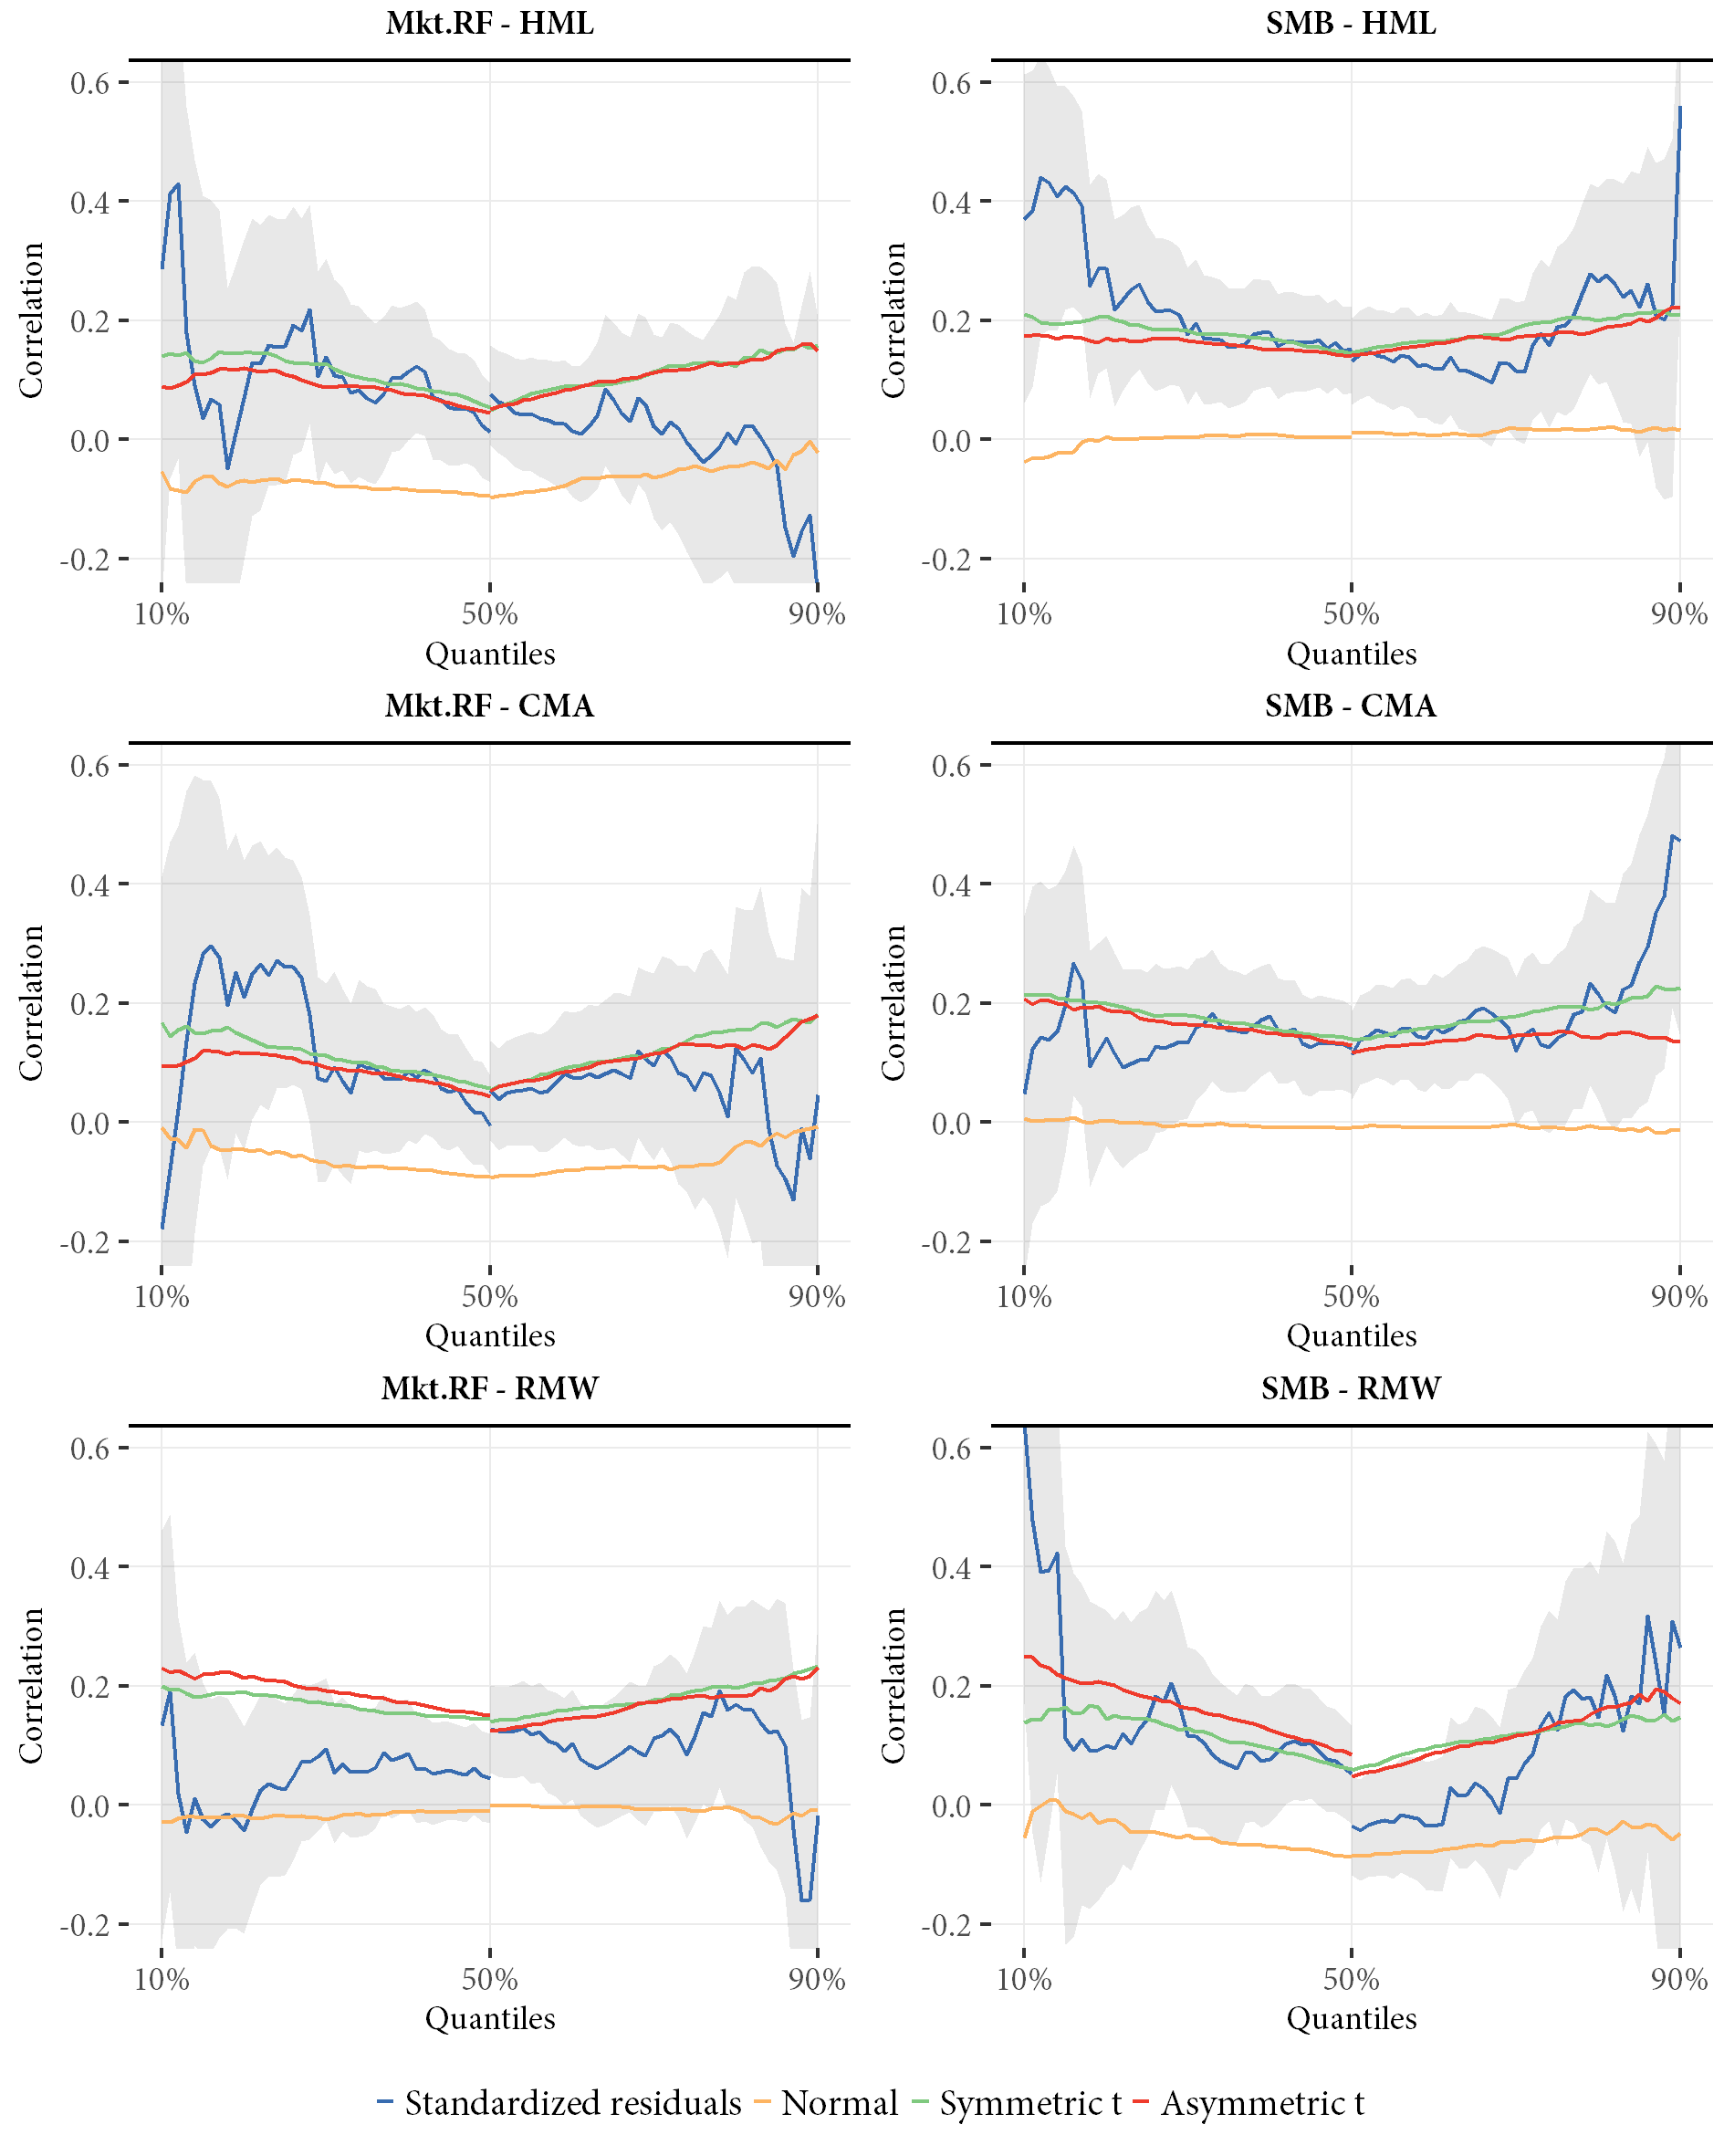
\includegraphics[scale=1]{graphics/threshold_simulated_1.png}  
  \footnotesize
  \caption{Threshold correlations of standardized residuals from the constant copulas}

  \begin{longcaption}
    Threshold correlations of simulated constant copulas, compared to ARMA-GARCH standardized residuals (95\% confidence bounds taking the ARMA-GARCH models as given). The simulated threshold correlations are based on 250,000 simulated returns each. ARMA-GARCH models based on empirical weekly data 1963--2016.
  \end{longcaption}
  \label{fig:threshold_simulated1}
\end{figure}
\pagebreak
\begin{figure}[!ht]
  \ContinuedFloat
  \centering
  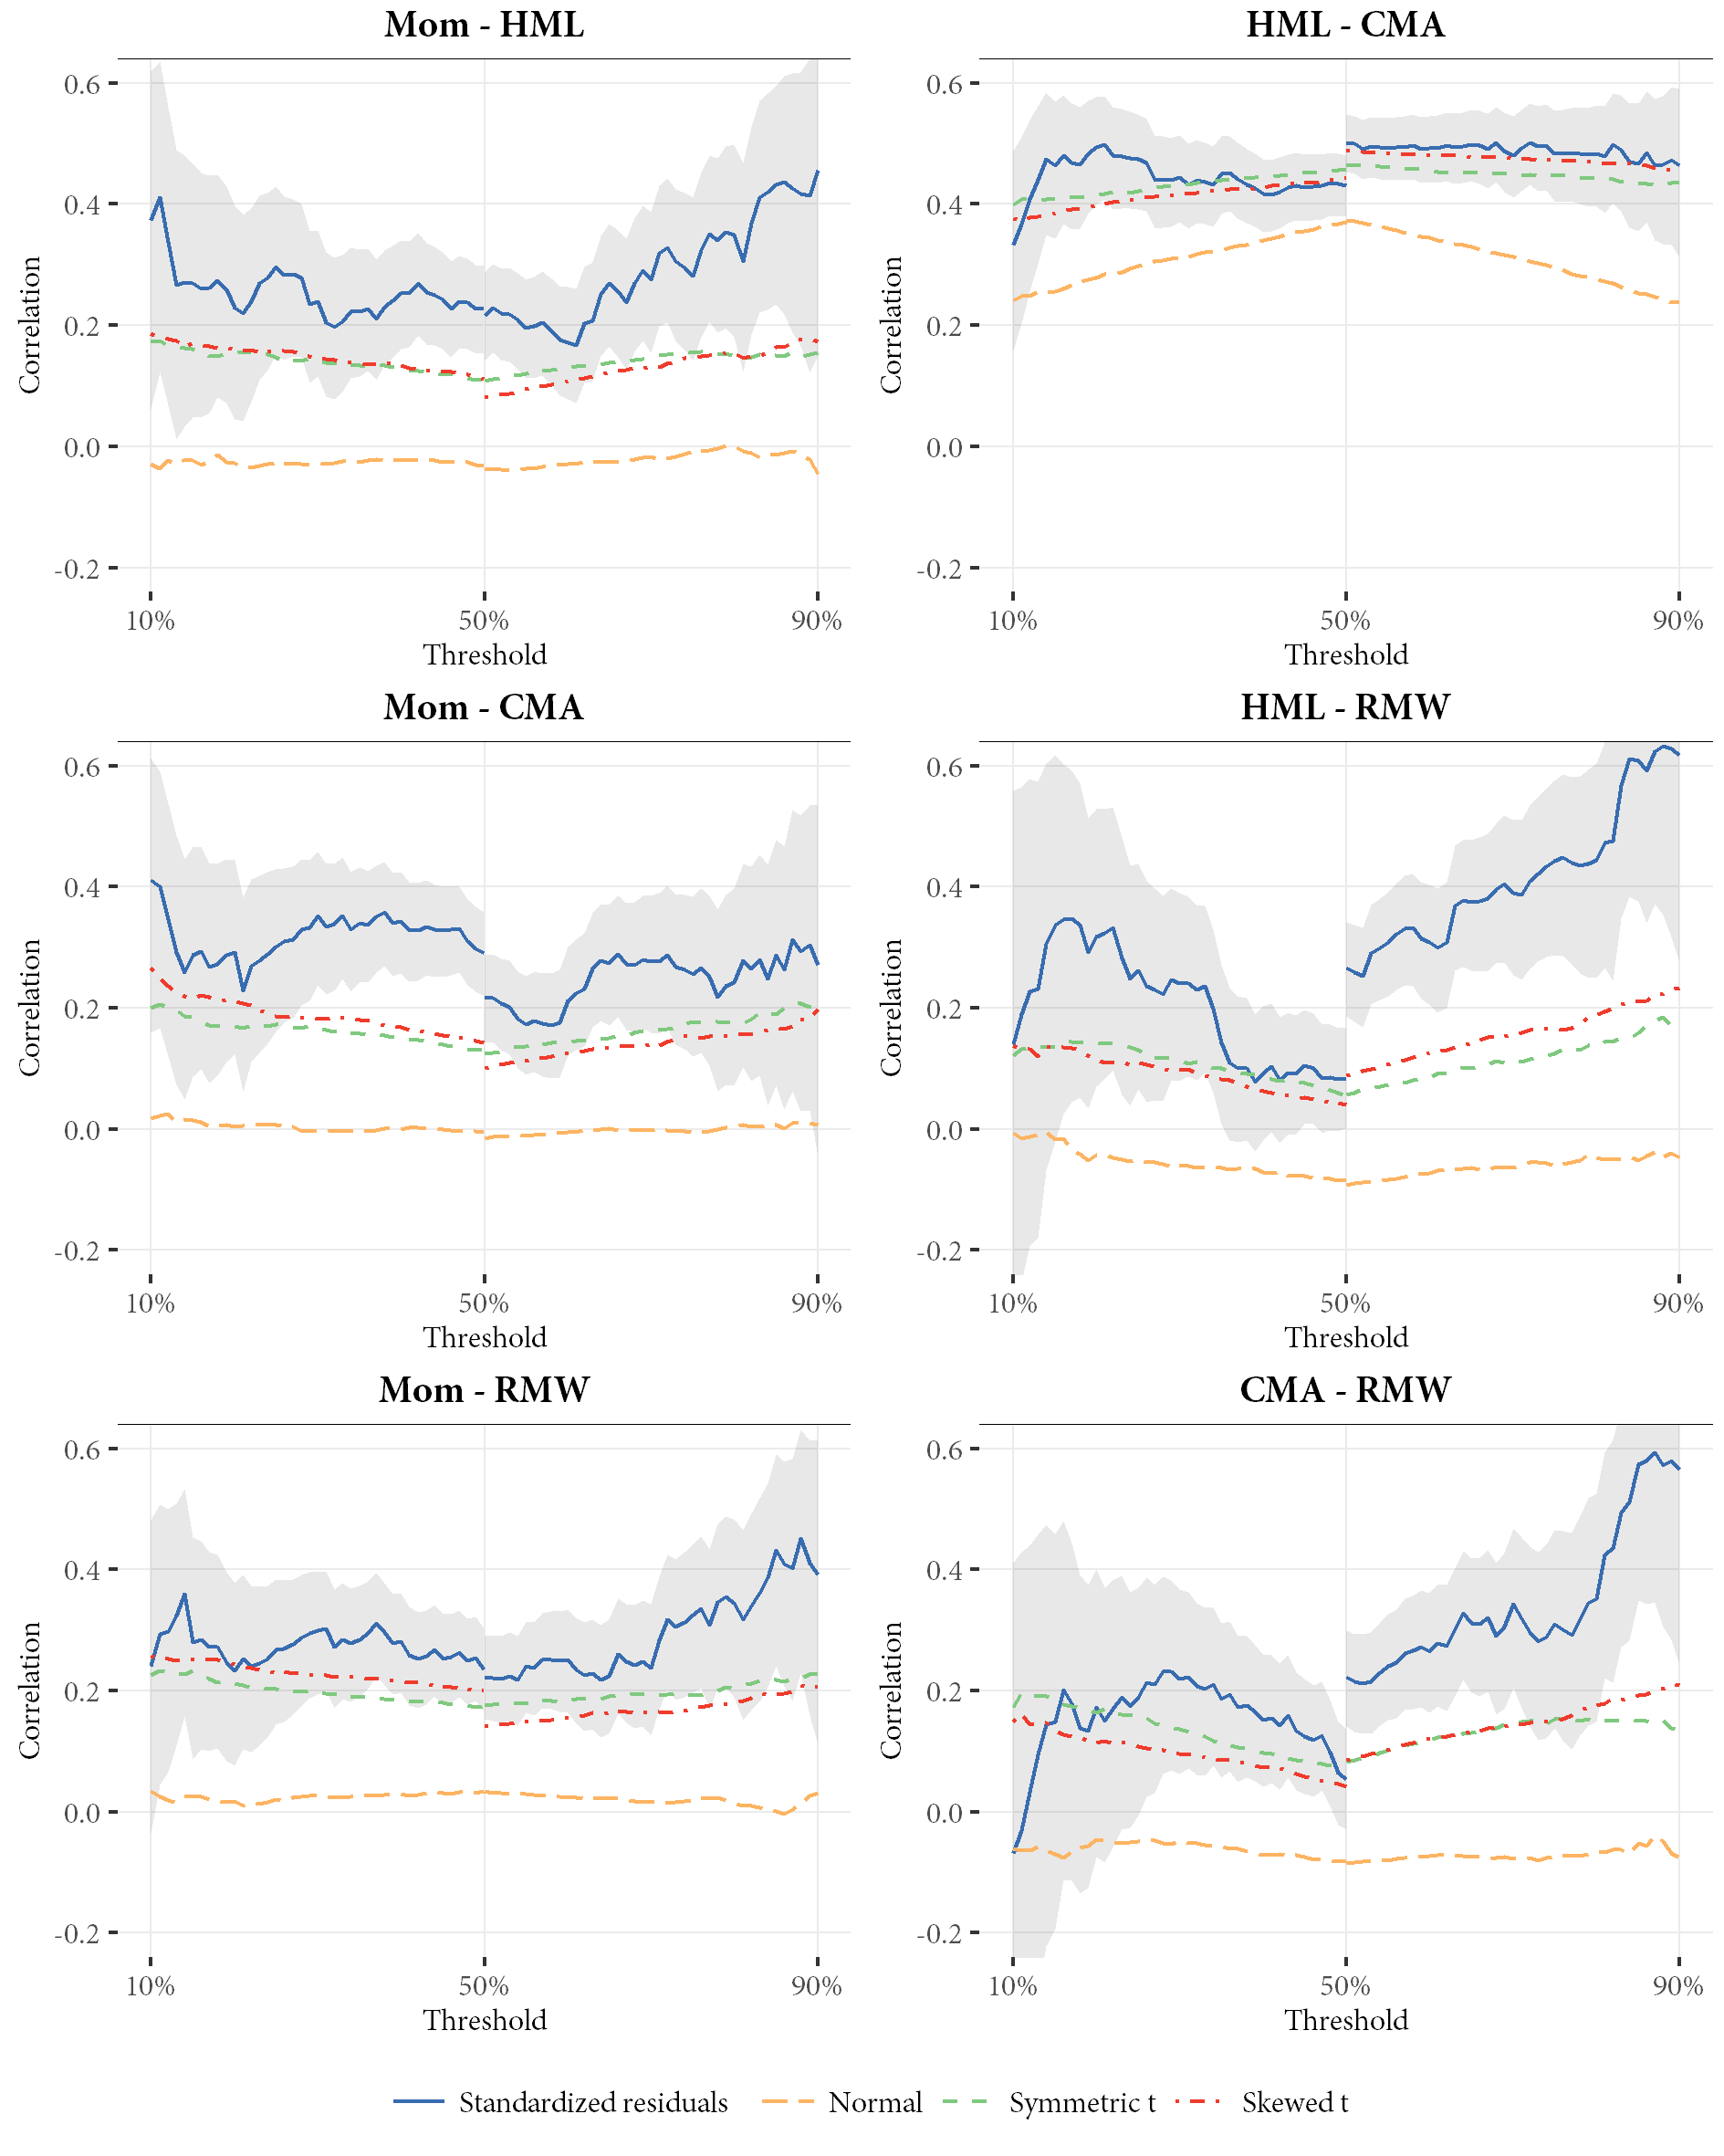
\includegraphics[scale=1]{graphics/threshold_simulated_2.png}  
  \footnotesize
  \caption{Threshold correlations of standardized residuals from the constant copulas (cont.)}
\end{figure}
\pagebreak

First, we note that for most factors, the normal copula is the far away from generating threshold correlations that correspond to the empirical distribution around the median. This is highly expected, as the normal copula does not generate tail dependence, and hence the need for the Student's \textit{t} based copula models. The symmetric \textit{t} and asymmetric \textit{t} copulas better capture the threshold correlations, as the fatter tails of the Student's \textit{t} distribution allows for tail dependence. For example, note how the normal copula generates negative threshold correlations for both the Mom--HML and RMW--HML asset pairs, while the Student's \textit{t} based copulas are much closer to the higher values in the data. On the other hand, the Student's \textit{t} based copulas sometimes seem to overshoot the empirical threshold correlation, as in the Mkt.RF--RMW asset pair.

Second, we find that the skewed Student's \textit{t} generates some asymmetry around the median, which can be seen most clearly for the Mom--RMW and RMW--HML asset pairs. The generated asymmetry does, however, appear to be too small to capture the features of the data.

In conclusion, comparing threshold correlations from empirical data and simulated data shows that the constant copula specifications capture some of the tail dependence.\footnote{Note that, in order to make the threshold correlation comparison valid, we use the constant copula specifications. The dynamic version is still the workhorse for all continued analysis in the mean-variance and diversification benefit sections.} Although the Student's \textit{t} and skewed Student's \textit{t} results do not align perfectly with the data, they constitute clear improvements to the normal copula in modeling tail dependence. We observe that the copula seems to lack flexibility to simultaneously generate all the asymmetries in tail dependence. This is quite expected, as the Student's \textit{t} copula only has one degree of freedom parameter that controls the fatness of tails, and the skewed Student's \textit{t} copula only has one skewness parameter for each series. This imposes limits on how strongly the model can express fat tails or asymmetries between factors A and B and simultaneously express other fat tails or asymmetries (or lack thereof) between factors A and C. For a collection of six factors with heterogenous dependence, this is even harder. This is a clear limitation of our quite parsimonious multivariate distribution copula approach. In this regard, vine copulas that allow for unique bivariate copula specifications, as discussed in \autoref{sub:05_01_choosing}, could be the solution.

Although imperfect, the multivariate copula modeling of tail dependence could constitute a significant improvement to alternatives, especially in the field of risk management, where understanding of tail events is paramount.

\subsubsection{Rolling correlations in the dynamic copula}

In-sample, we simulate 10,000 standardized residuals for each week from the estimated dynamic symmetric Student's \textit{t} copula model, and compute the rolling 52-week correlations. This is done to ascertain ourselves that the chosen copula specification does in fact capture the time-variation in correlations. The comparison is made between standardized residuals from the simulated copula model and standardized residuals from the ARMA-GARCH model of univariate series. If satisfactory, the rolling correlations of the copula model and the ARMA-GARCH univariate models will be roughly the same.

\begin{figure}[!ht]
  \centering
  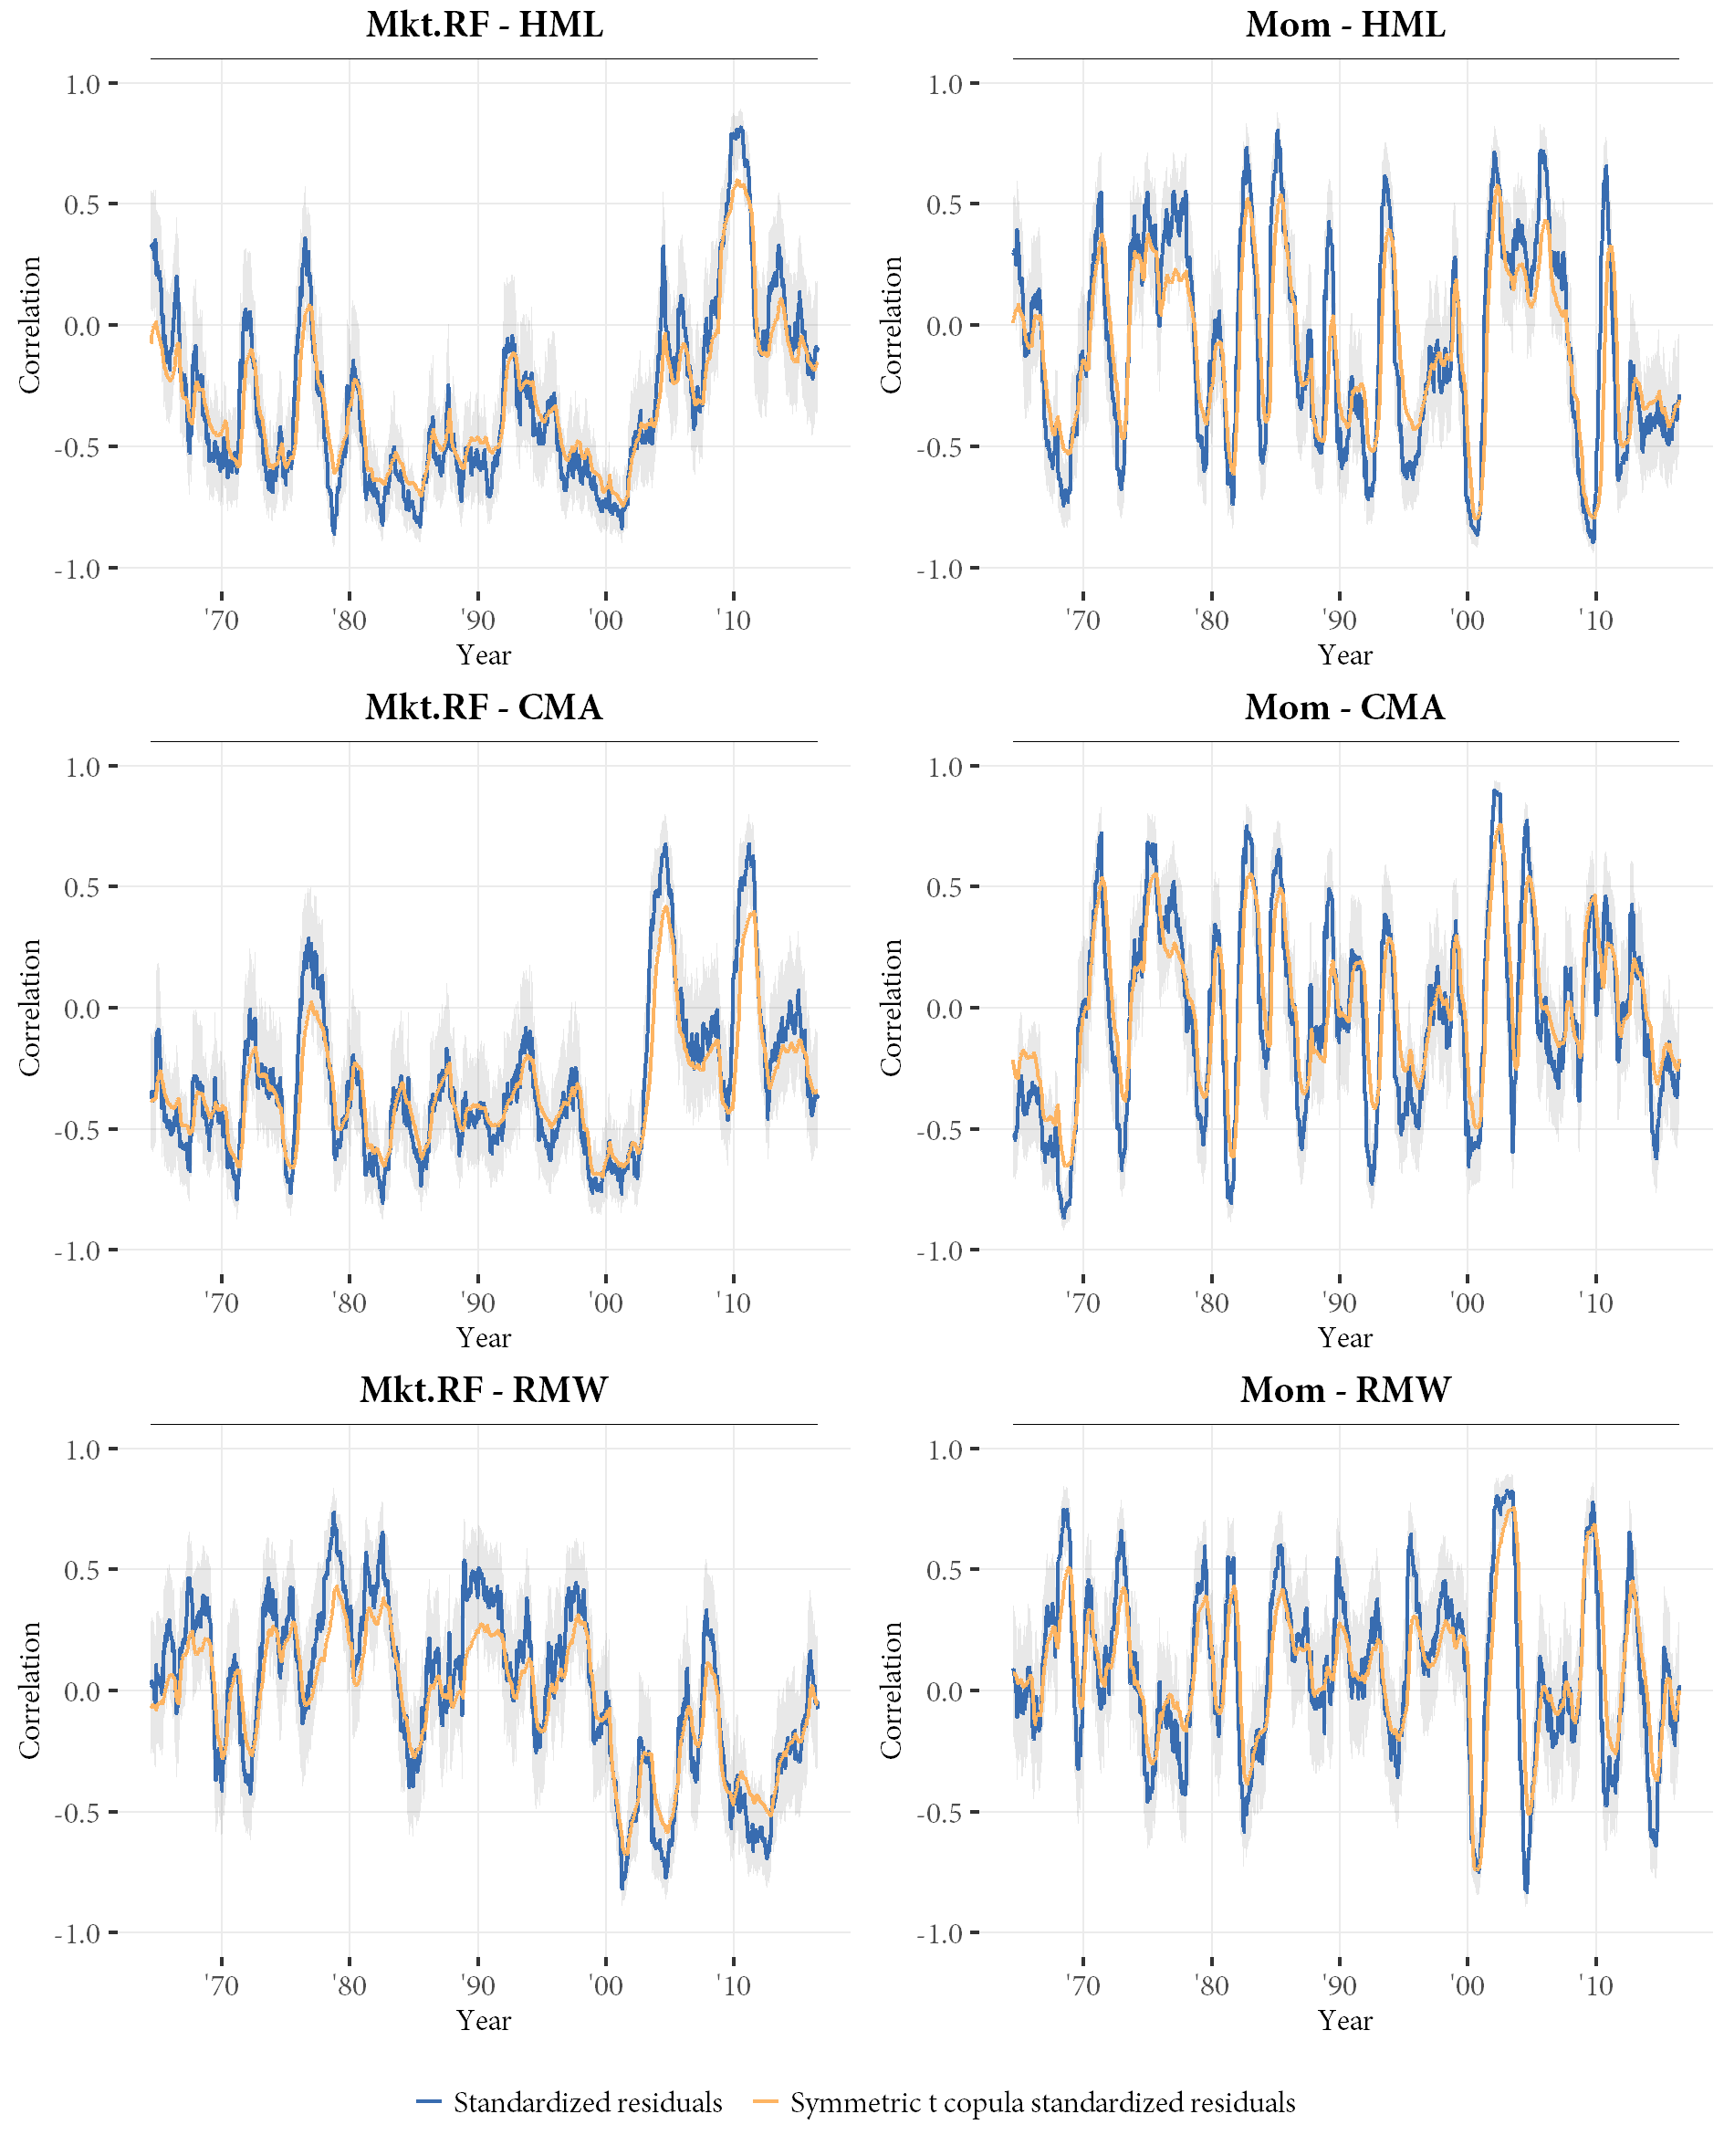
\includegraphics[width=\textwidth]{graphics/rolling_simulated1.png}
  \footnotesize
  \caption{Rolling correlations of standardized residuals from the dynamic copula}

  \begin{longcaption}
    Rolling correlations of the simulated dynamic symmetric \textit{t} copula compared to rolling correlations on ARMA-GARCH residuals. 95\% confidence bounds taking the ARMA-GARCH models as given. The simulated rolling correlations are based on 10,000 simulations each week. ARMA-GARCH models based on empirical weekly data 1963--2016.
  \end{longcaption}
  \label{fig:rolling_simulated}
\end{figure}
\begin{figure}[!ht]
  \ContinuedFloat
  \centering
  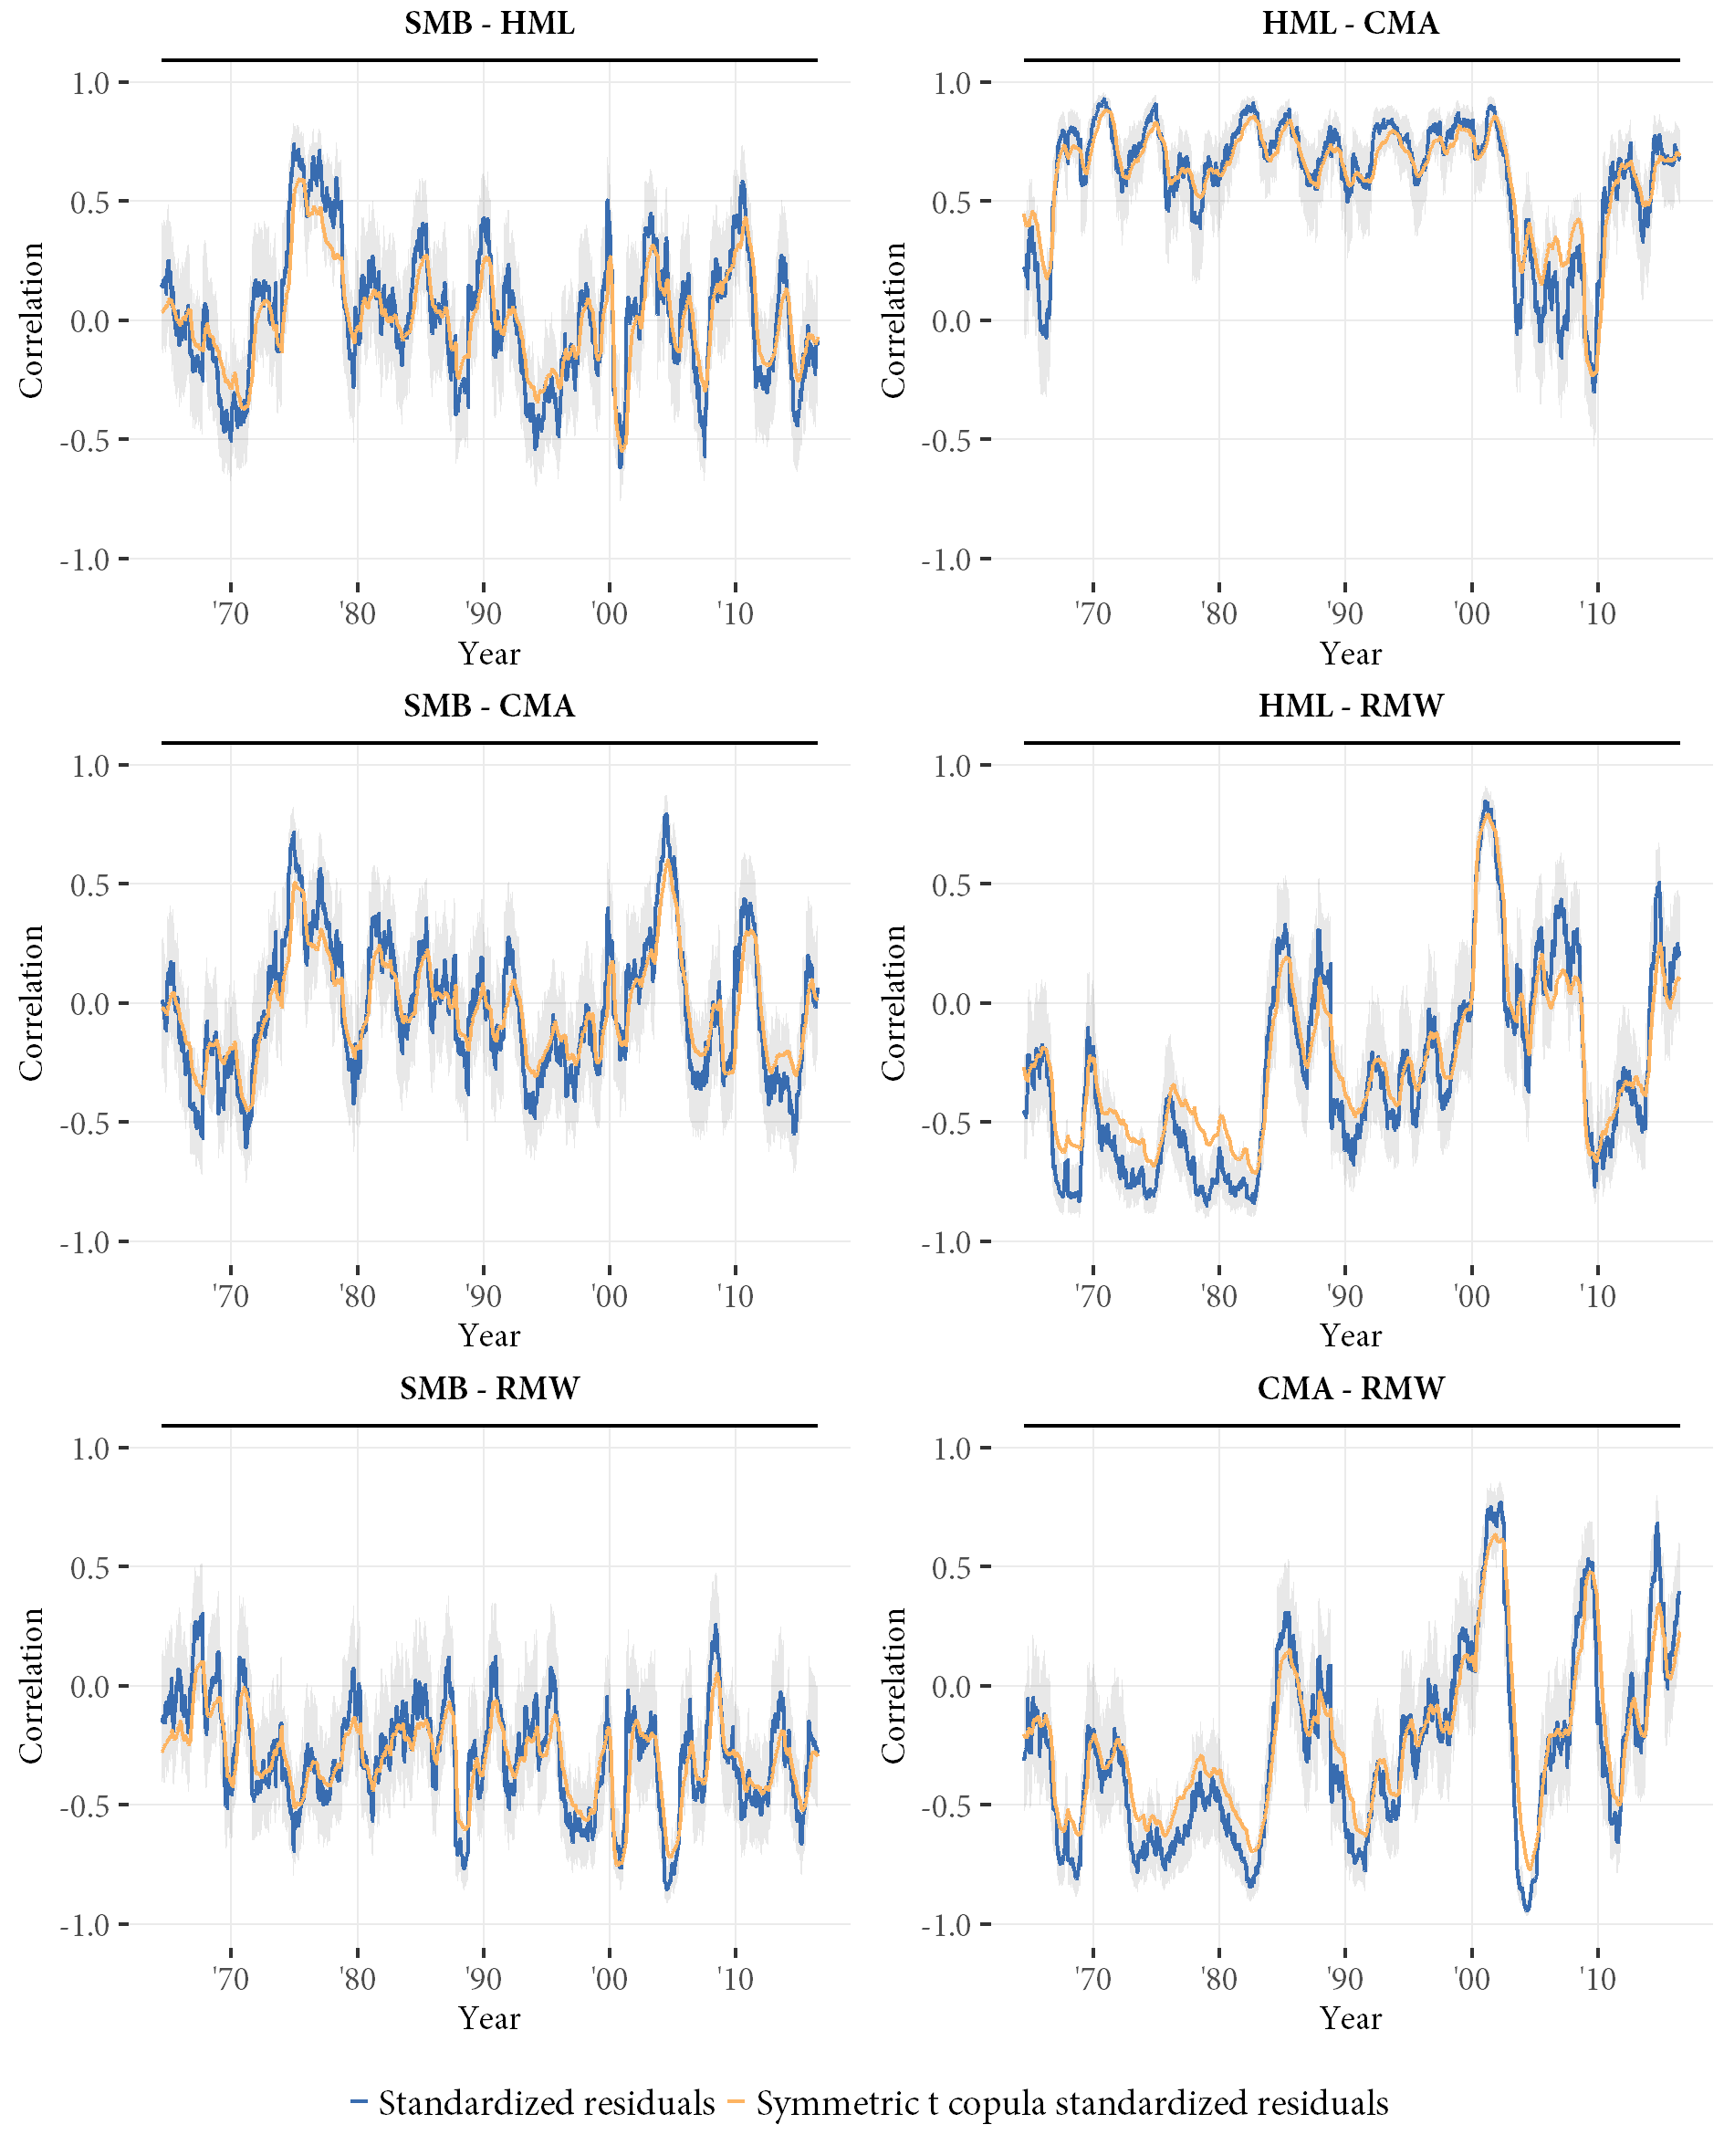
\includegraphics[width=\textwidth]{graphics/rolling_simulated2.png}
  \footnotesize
  \caption{Rolling correlations of standardized residuals from the dynamic copula (cont.)}
\end{figure}

While we do not get a perfect overlap, the copula model generates similar time-varying correlations. When there are large swings, however, the model does not always have enough amplitude. We conclude that the model captures the dynamic features well. % constant threshold corrs simulated, maybe also add robustness check of whether the model captures roll-corrs 

% section modeling_of_factor_returns (end)
